\documentclass[12pt,a4paper,parskip=full]{scrartcl}
\usepackage{float}
% \usepackage{bbding}
% \usepackage{pifont}
% \usepackage{wasysym}
%\usepackage[default,scale=1]{opensans} 
\usepackage{xeCJK}
\setCJKmainfont{IPAGothic}
%\usepackage[T1]{fontenc}
\usepackage[margin=1in]{geometry}
\geometry{letterpaper}
\usepackage{xcolor}
\definecolor{red}{HTML}{cc0000}
\definecolor{gray}{HTML}{666666}
\usepackage{sectsty}
\sectionfont{\color{red}}
%\subsectionfont{\fontsize{25}{25}\color{red}}
\subsectionfont{\color{red}}
%\subsubsectionfont{\fontsize{20}{20}\color{red}}
\subsubsectionfont{\color{red}}
\usepackage{graphicx}
\usepackage{hyperref}
%\usepackage{amssymb}
\usepackage[style=footnote-dw]{biblatex}
\bibliography{S@SGuideBib}
\setlength\bibitemsep{0.5\baselineskip}
\graphicspath{{./images/}}

\usepackage{enumitem}
%\setitemize{noitemsep}
% \setlist{noitemsep, topsep=-5pt}
% \setlength\itemsep{-0.10em}

\renewcommand{\labelitemi}{$\cdot$}
\renewcommand{\labelitemii}{$\cdot$}
\makeatletter
\let\latexl@section\l@section
\def\l@section#1#2{\begingroup\let\numberline\@gobble\latexl@section{#1}{#2}\endgroup}
\makeatother

\usepackage[T1]{fontenc}
\fontfamily{verdana}

%\usepackage{scrlayer-scrpage}{}
\usepackage{fancyhdr}
\makeatletter
\renewcommand{\@seccntformat}[1]{}
\makeatother

\setlength\parindent{0pt}{}

\pagestyle{fancy}
\fancyhf{}
\iffalse
\lhead{ \fancyplain{}{The Scrum@Scale Guide}}
\fi
\lhead{ \fancyplain{}{Scrum@Scaleガイド}}
\rfoot{ \fancyplain{}{\thepage} }
\lfoot{\textcopyright 2006-2021 Jeff Sutherland \& Scrum Inc.}



\title{\Huge{\color{red}\textbf{The Scrum@Scale 
\textsuperscript{\registered} 
Guide}}}
\subtitle{\color{gray}The Definitive Guide to Scrum@Scale:\\ Scaling that Works}
% \author{}
\date{}




\begin{document}
\tableofcontents
\iffalse
\subsection{Preface to the Scrum@Scale
Guide}\label{preface-to-the-ScrumatScale-guide}
\fi
\subsection{Scrum@Scaleガイドの序文}\label{preface-to-the-ScrumatScale-guide}

\iffalse
Scrum, as originally outlined in the Scrum Guide, is focused on a single Scrum Team being able to deliver optimal value while maintaining a sustainable pace. Since its inception, the usage of Scrum has extended to the creation of products, processes, and services that require the efforts of multiple teams. 
\fi
スクラムは、もともとスクラムガイドで説明されているように、単一のスクラムチームが、持続可能なペースを維持しつつ、最適な価値を提供できるようにすることを重視している。スクラムガイドの発行以降、スクラムの利用はプロダクト、プロセス、サービスなどの開発といった複数チームの協力が求められる領域まで広がりを見せている。

\iffalse
In the field, it was repeatedly observed that as the number of Scrum Teams within an organization grew, two major issues emerged:
\fi
現場では、組織内のスクラムチーム数の増加に伴い、2つの重要な問題の発生が繰り返し見られた。

\begin{itemize}%[label={\huge\textbullet}]
\itemsep10pt
\iffalse
\item
  The volume, speed, and quality of their output (working product) per team began to fall, due to issues such as cross-team dependencies, duplication of work, and communication overhead 
\item
 The original management structure was ineffective for achieving business agility. Issues arose like competing priorities and the inability to quickly shift teams around to respond to dynamic market conditions
\fi
\item
複数のチームの間での依存関係や作業の重複、コミュニケーションのオーバーヘッドなどの問題により、チームごとのアウトプット(動作するプロダクト)の量、スピード、品質が低下し始めた。
\item
従来の組織構造はビジネスアジリティの実現に十分な効果を上げられなかった。優先順位の競合や、市場の変化に対応するようチームを素早く転換させることができないなどの問題が発生した。
\end{itemize}

\iffalse
To counteract these issues, a framework for effectively coordinating multiple Scrum Teams was clearly needed which would aim for the following:
\fi
こうした問題に対処するために、複数のスクラムチームを効果的に調整するフレームワークが明らかに必要だった。Scrum@Scaleフレームワークの目的は以下の通り。

\begin{itemize}
\itemsep10pt
\iffalse
\item
  Linear scalability: A corresponding percentage increase in delivery of working product with an increase in the number of teams
\item
 Business agility: The ability to rapidly respond to change by adapting the initial stable configuration
\fi
\item
リニアなスケーラビリティ: チーム数の増加に比例して、動作するプロダクトのデリバリーも増加する
\item
ビジネスアジリティ: 初期の安定した構成を適応させることで、変化に素早く対応できる
\end{itemize}

\iffalse
Scrum@Scale helps an organization to focus multiple networks of Scrum Teams on prioritized goals. It aims to achieve this by setting up a structure which naturally extends the way a single Scrum Team functions across a network and whose managerial function exists within a minimum viable bureaucracy (MVB).
\fi
Scrum@Scaleは、複数のスクラムチームのネットワークが、組織において優先順位付けされたゴールに集中するのに役立つ。Scrum@Scaleの目的は、単一のスクラムチームが機能するやり方を複数のチームのネットワーク全体へと自然に拡大し、管理機能が実用最小限の官僚機構(MVB)内にある、という構造を構築することである。

\iffalse
A network can achieve linear scalability when its characteristics are independent of its size. Designing and coordinating a network of teams with this goal does not constrain growth in a particular way; instead, it allows for the network to grow organically, based on its unique needs, and at a sustainable pace of change that can be better accepted by the individuals involved.
\fi
チームのネットワークの特性がそのサイズに依存しない場合、リニアなスケーラビリティを実現できる。このゴールのためにチームのネットワークを設計・調整することは、特定の方法で成長を制約するものではない。むしろ、ネットワークが独自のニーズに基づいて有機的に成長することを可能にし、関係者に受け入れられやすい持続的な変化のペースを実現する。

\iffalse
A minimum viable bureaucracy is defined as having the least amount of governing bodies and processes needed to carry out the function(s) of an organization without impeding the delivery of customer value. It helps to achieve business agility by reducing decision latency (time to make a decision), which has been noted as a primary driver of success. In order to begin implementing Scrum@Scale, it is essential to be familiar with the Agile Manifesto and the 2020 Scrum Guide. A failure to understand the nature of agility will prevent it from being achieved. If an organization cannot Scrum, it cannot scale.
\fi
実用最小限の官僚機構とは、顧客に価値を届けるのを妨げることなく、組織を機能させるために必要な機関とプロセスが最小限であるものと定義される。意思決定の遅延を減らすことは、ビジネスアジリティの実現に役立つ。このことは、成功の主な原動力として知られている。Scrum@Scaleの導入を開始するには、アジャイルマニュフェストとスクラムガイド2020をよく理解することが不可欠である。アジリティの本質を理解しないと、それを達成することはできない。スクラムを実践できない組織は、スケールすることはできない。


\iffalse
\subsection{Purpose of the Scrum@Scale
Guide}\label{purpose-of-the-ScrumatScale-guide}
\fi
\subsection{Scrum@Scaleガイドの目的}\label{purpose-of-the-ScrumatScale-guide}

\iffalse
This guide provides the definition of Scrum@Scale and the components of its framework. It explains the accountabilities of the scaled roles, scaled events, and enterprise artifacts, as well as the rules that bind them together.
\fi
このガイドは、Scrum@Scaleと、そのフレームワークのコンポーネントの定義を提供する。そして、スケールされた役割、スケールされたイベント、エンタープライズにおける作成物に対する責任と、それらを結び付けるルールについて説明する。

\iffalse
This guide is broken down into four basic sections:
\fi
このガイドは次の4つのセクションに大きく分割されている。

\begin{itemize}
\itemsep1pt\parskip0pt\parsep0pt
\iffalse
\item
  an introduction to Scrum@Scale, with the basics for getting started
\item
  an overview of the Scrum Master Cycle
\item
  an overview of the Product Owner Cycle
\item
  a walk-through of bringing the cycles together
\fi
\item
Scrum@Scaleを始めるための基本
\item
スクラムマスターサイクルの概要
\item
プロダクトオーナーサイクルの概要
\item
2つのサイクルを結び付けるウォークスルー
\end{itemize}

\iffalse
Each component serves a specific purpose which is required for success at scale. Changing their core design or ideas, omitting them, or not following the base rules laid out in this guide limits the benefits of Scrum@Scale.
\fi
スケーリングの成功には各コンポーネントが必要となる。それらの中核となる設計思想を変更したり、省略したりすると、あるいは、本ガイドに示す基本的なルールに従わないと、Scrum@Scaleのメリットを享受できない。

\iffalse
Specific tactics beyond the basic structure and rules for implementing each component vary and are not described in this Guide. Other sources provide complementary patterns, processes, and insights.
\fi
基本的な構造とルール以外の各コンポーネントを実装する具体的な戦術はさまざまであるため、本ガイドには記載していない。補足的なパターン、プロセス、インサイトは、その他の情報源で提供されている。

\iffalse
\subsection{Definitions}\label{definitions}
\fi
\subsection{定義}\label{definitions}

\iffalse
Scrum is a lightweight framework that helps people, teams and organizations generate value through adaptive solutions for complex problems.
\fi
スクラムとは、複雑な問題に対応する適応型のソリューションを通じて、人々、チーム、組織が価値を生み出すための軽量級フレームワークである。

\iffalse
The Scrum Guide describes the minimal set of elements that create a team environment that drives innovation, customer satisfaction, performance, and happiness. Scrum utilizes radical transparency and a series of formal events to provide opportunities to inspect and adapt a team and its product(s).
\fi
スクラムガイドでは、イノベーション、顧客満足、パフォーマンス、幸福を促進するチーム環境を生み出す要素の最小限のセットについて説明している。スクラムは、徹底的な透明性と一連の公式なイベントを使い、チームとそのプロダクトを検査・適応する機会を提供する。

\iffalse
Scrum@Scale is a lightweight organizational framework in which a network of teams operating consistently with the Scrum Guide can address complex adaptive problems, while creatively delivering products of the highest possible value. These ``products'' may be physical, digital, complex integrated systems, processes, services, etc.
\fi
Scrum@Scaleは、スクラムガイドに従って機能しているチームのネットワークが、複雑適応系の問題に対処しつつ、最高の価値のプロダクトを創造的にデリバリーすることを可能とする、軽量級の組織フレームワークである。これらの「プロダクト」としては、物理的、デジタル、または複雑な統合システム、プロセス、サービスなどがある。

\iffalse
The Scrum@Scale Guide describes the minimal set of components to scale Scrum by using Scrum and its resulting business agility across an entire organization. It can be used in all types of organizations within industry, government, nonprofits, or academia. If an organization does not already use Scrum, it will require changes to its operating system.
\fi
Scrum@Scaleガイドでは、スクラムを利用してスクラムをスケールするための最小限のコンポーネントセットと組織全体で生まれるビジネスアジリティーについて説明している。本ガイドは、産業界、政府、非営利団体、学界のあらゆるタイプの組織で活用できる。スクラムをまだ使っていない組織では、組織のオペレーティングシステムを変更する必要がある。

\iffalse
In Scrum, care is taken to separate accountability of the ``what'' (product) from the ``how'' (process). The same care is taken in Scrum@Scale, so that jurisdiction and accountability are expressly understood. This eliminates wasteful organizational conflict that keep teams from achieving their optimal productivity. Because Scrum@Scale consists of components, it allows an organization to customize their transformation strategy and implementation. It gives an organization the ability to target incrementally prioritized change efforts in the area(s) deemed most valuable or most in need of adaptation and then progress on to others.
\fi
スクラムでは、"What"(プロダクト)と"How"(プロセス)の責任の分離に注意する必要がある。Scrum@Scaleでも、管轄と責任が明確に理解されるように、同じ注意が払われる。これにより、チームがその最適な生産性を達成するのを邪魔する、無駄な組織上の衝突が取り除かれる。Scrum@Scaleはコンポーネントで構成されているため、組織はその変革の戦略と実施をカスタマイズできる。これにより、組織は、最も価値がある、あるいは最も適応が必要であると考えられる分野に、段階的に優先順位をつけて変革の取り組みを行い、その後、他の分野に進むことができる。

\iffalse
Scrum@Scale separates these components into two cycles: the Scrum Master Cycle (the ``how'') and the Product Owner Cycle (the ``what''), intersecting at two components and sharing a third. Taken as a whole, these cycles produce a powerful supporting structure for coordinating the efforts of multiple teams along a single path.
\fi
Scrum@Scaleは、これらのコンポーネントを、スクラムマスターサイクル(“How”)とプロダクトオーナーサイクル(“What”)に分け、この2つのサイクルが2つのコンポーネントで交わり、3つ目のコンポーネントを共有する。まとめると、これらのサイクルは、一つの道筋に沿って複数のチームの取り組みを調整することを強力にサポートする構造を作り出す。

\iffalse
\subsection{The Components of
Scrum@Scale}\label{the-components-of-scrumatscale}
\begin{figure}[H]
    \centering
    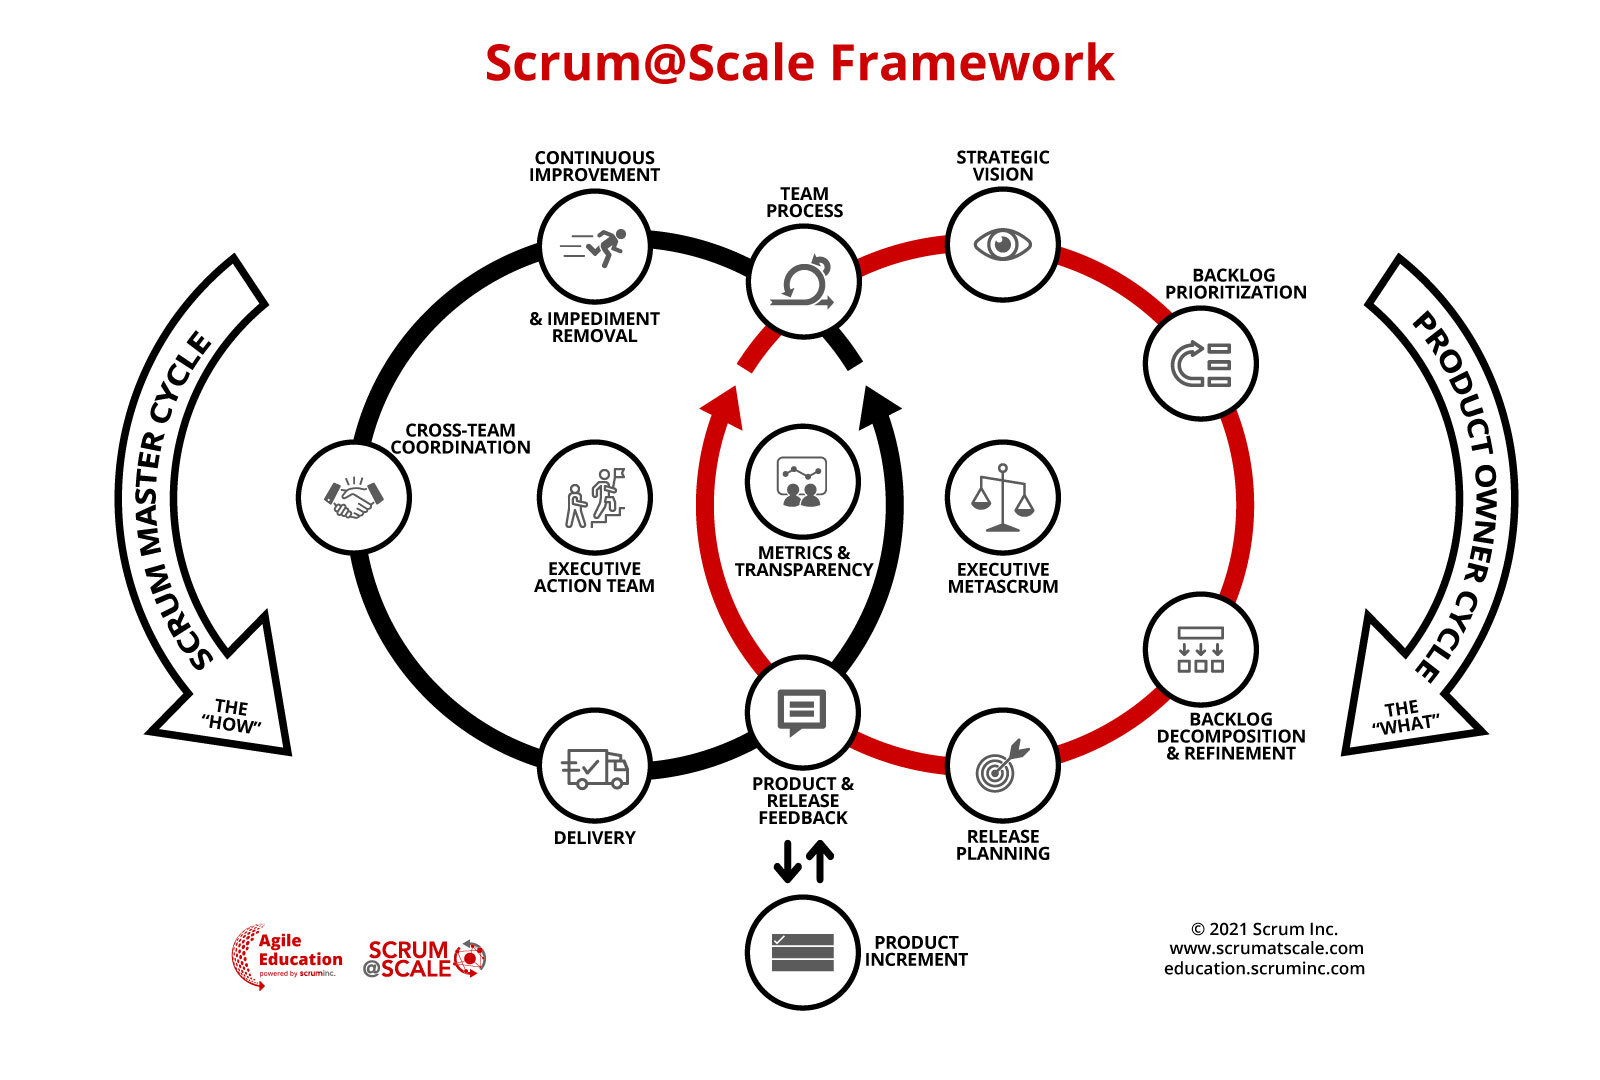
\includegraphics[scale=0.25]{SMPO-Cycle.png}
\end{figure}
\fi
\subsection{Scrum@Scaleのコンポーネント}\label{the-components-of-scrumatscale}
\begin{figure}[H]
    \centering
    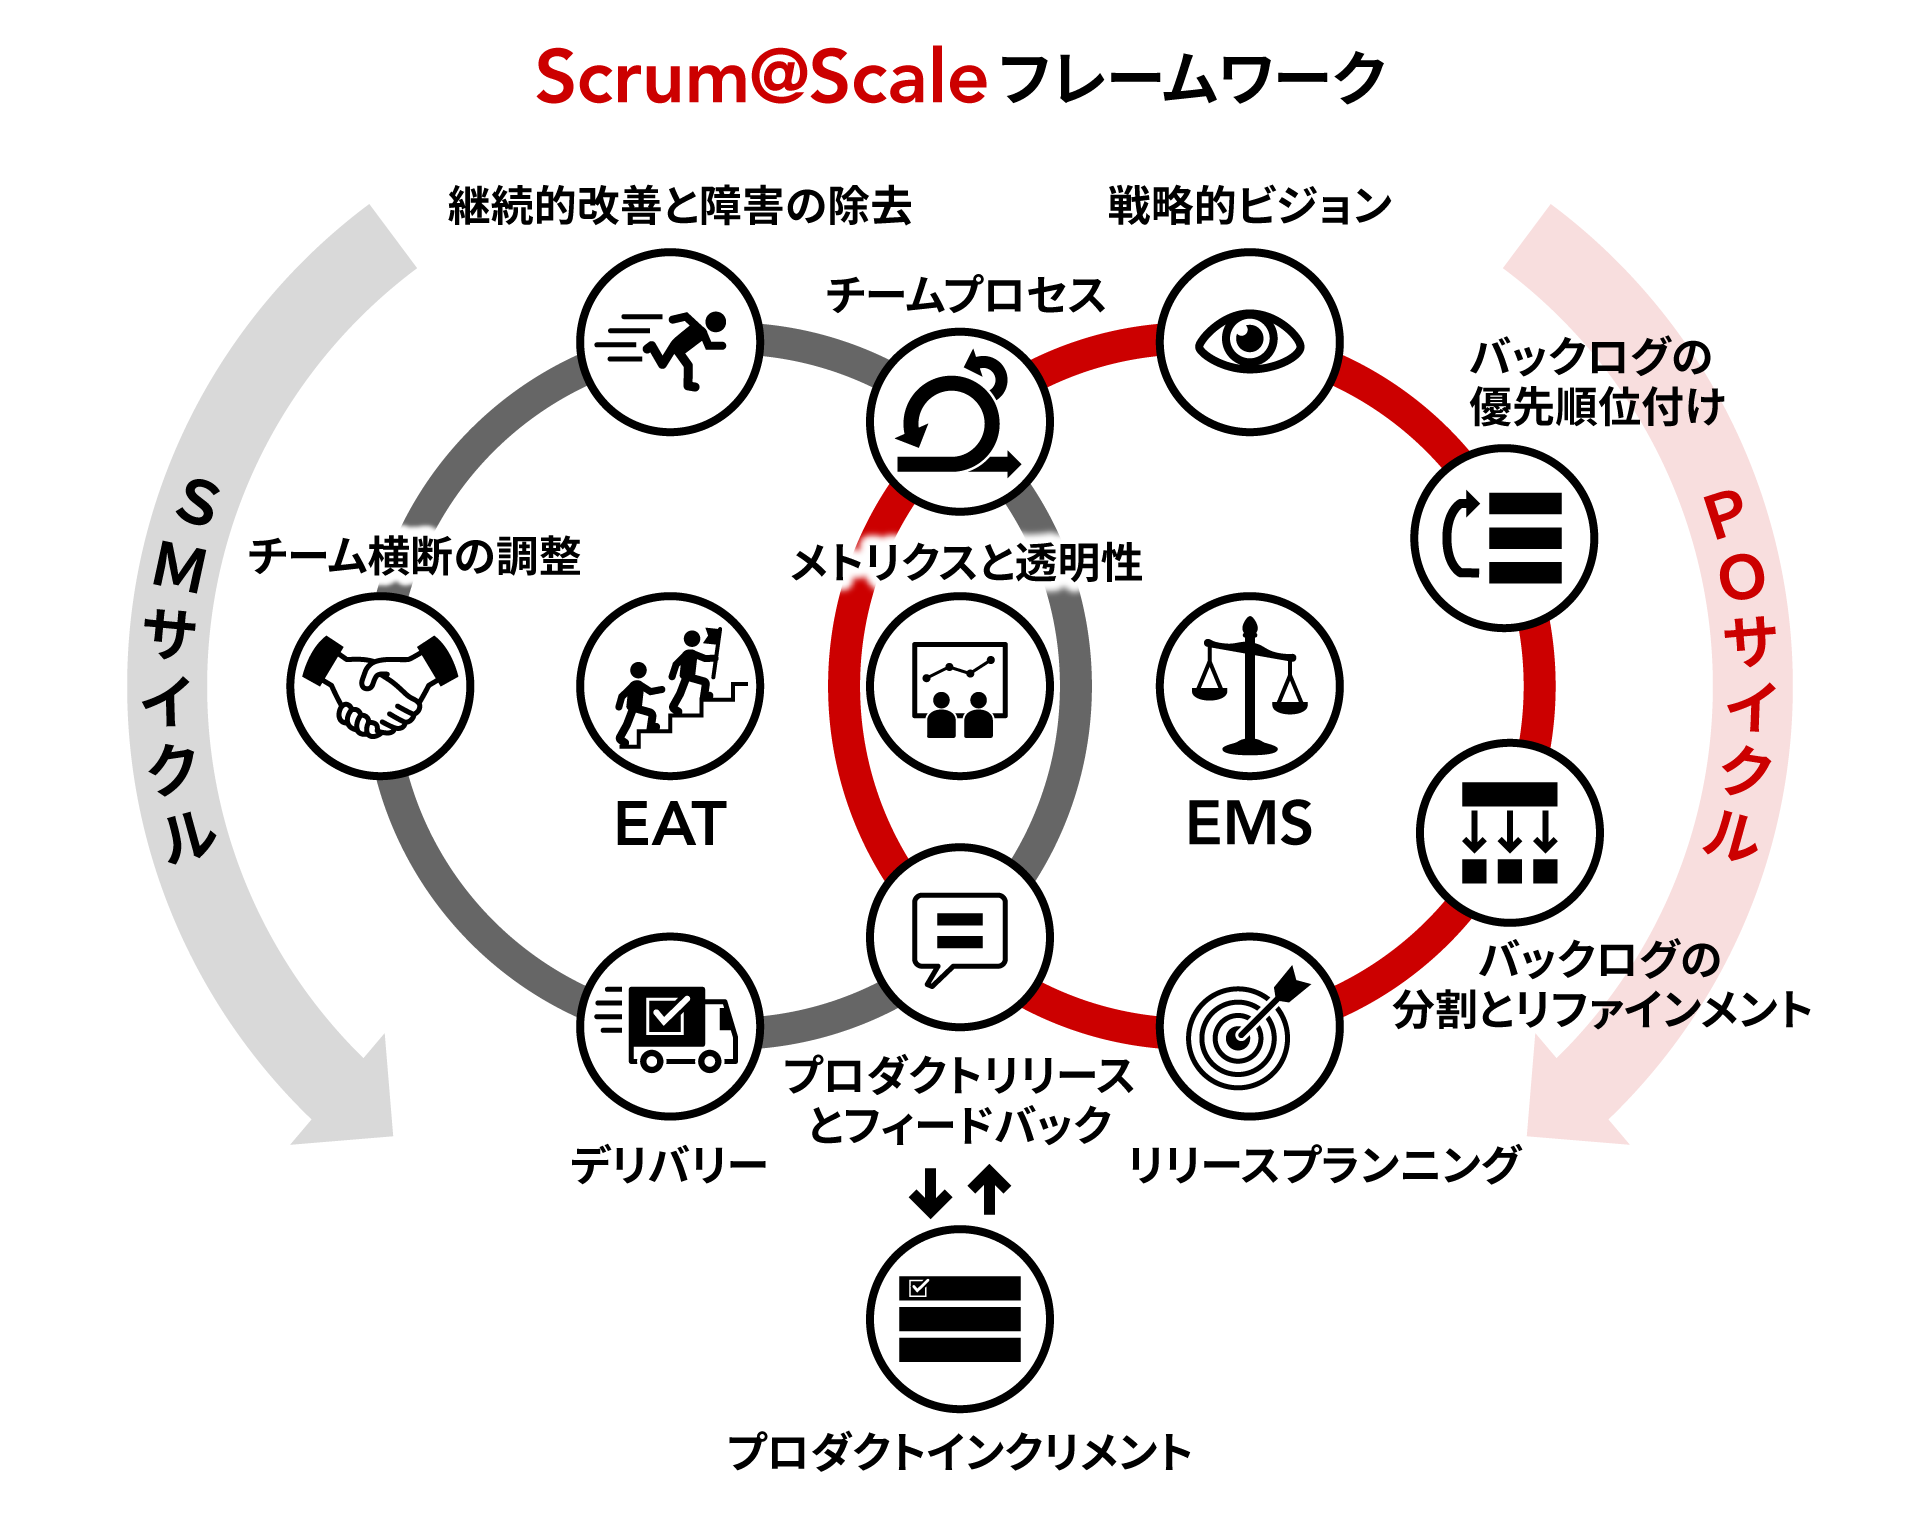
\includegraphics[scale=0.25]{SMPO-Cycle-JA.png}
\end{figure}

\iffalse
\subsubsection{Values-Driven Culture}\label{values-driven-culture}
\fi
\subsubsection{価値駆動文化}\label{values-driven-culture}

\iffalse
Scrum@Scale aims to build a healthy organizational culture through the pillars of empirical process control and the Scrum Values. The pillars of empirical process control are transparency, inspection, and adaptation.  These pillars are actualized by the Scrum values of Openness, Courage, Focus, Respect, and Commitment.
\fi
Scrum@Scaleの目的は、経験的プロセス制御の柱とスクラムの価値基準を通じて健全な組織文化を構築することである。経験的プロセス制御の三本柱とは、透明性、検査、適応である。これらの柱は、公開(オープン性)、勇気、集中、尊敬、確約(コミットメント)というスクラムの価値基準によって現実のものとなる。

\iffalse
Openness supports transparency into all of the work and processes and without it, there is no ability to inspect them honestly and attempt to adapt them for the better. Courage refers to taking the bold leaps required to deliver value quicker in innovative ways. Focus and Commitment refer to the way we handle our work obligations, putting customer value delivery as the highest priority. Lastly, all of this must occur in an environment based on respect for the individuals doing the work, without whom nothing can be created.
\fi
公開(オープン性)は、すべての作業とプロセスへの透明性を保証する。さもなくば誠実な検査と、より良いものに適合することはできない。勇気は、革新的な方法で、より迅速に価値を届けるために必要となる、大胆な飛躍をすることを示す。集中と確約(コミットメント)は、自分たちで自分たちの責務を全うする方法を見つけることを示し、顧客へ価値を届けることを最優先とするということである。最後に、これらすべては、他の誰も成しえない仕事に従事する個人への尊敬に支えられた環境なくしては成しえない。

\iffalse
Scrum@Scale helps organizations thrive by supporting a positive team learning environment for working at a sustainable pace, while putting customer value at the forefront.
\fi
Scrum@Scaleは、顧客価値の提供を最前線に置きつつ、持続可能なペースで仕事をする積極的なチームの学習環境をサポートする。これにより、組織の成長を支援する。


\iffalse
\subsubsection{Getting Started: Installing an Agile Operating
System}\label{getting-started-installing-an-agile-operating-system}
\fi
\subsubsection{Scrum@Scaleの始め方: アジャイルオペレーティングシステムを導入する}\label{getting-started-installing-an-agile-operating-system}

\iffalse
When implementing networks of teams, it is critical to develop a scalable Reference Model prior to scaling. The reference model is a small set of teams that coordinate to deliver every Sprint. As these teams successfully implement Scrum, the rest of the organization has a functioning, healthy example of Scrum to replicate. It serves as a prototype for scaling Scrum across the next network of teams. Any deficiencies in a Scrum implementation will be magnified when multiple teams are deployed. Scaling problems include organizational policies and procedures or development practices that block performance and frustrate teams.
\fi
チームのネットワークを導入する際は、スケールする前に、スケール可能なリファレンスモデルを開発することが不可欠である。リファレンスモデルは、スプリントごとにデリバリーを行うための調整を行う、小さなチームのセットである。これらのチームへのスクラムの導入が成功すると、機能する健全なスクラムの例ができ、組織の他のチームでも再現できるようになる。これは、チームの次のネットワークでスクラムをスケールするためのプロトタイプになる。多数のチームが同時に展開されると、スクラム導入における欠陥は拡大される。スケーリングの問題としては、パフォーマンスを阻んでチームに不満を抱かせるような組織の方針や手続き、開発手法などがある。

\iffalse
In a scaled setting, the Reference Model is best enabled by grouping teams together that need to coordinate in order to deliver a fully integrated set of Increments into a Scrum of Scrums (SoS). To operate effectively, the Scrum of Scrums needs to be supported by a minimum viable bureaucracy composed of two leadership groups: an Executive MetaScrum (EMS) forum, focused on what is produced by the Scrum of Scrums and an Executive Action Team (EAT) focused on how they can get it done faster. The Executive MetaScrum and Executive Action Team components are the hubs around which each cycle revolves.
\fi
スケールされた状況では、完全に統合された一連のインクリメントを提供するために調整が必要なチームをグループ化して、スクラムオブスクラム(SoS)にすることで、リファレンスモデルが最も有効になる。スクラムオブスクラムを効果的に運用するためには、2つのリーダーシップグループで構成された、実用最小限の官僚機構によってサポートされる必要がある。実用最小限の官僚機構とは、スクラムオブスクラムによって何を生み出すべきかに焦点を当てたエグゼクティブメタスクラム(EMS)フォーラムと、どのようにスクラムオブスクムにより速く仕事を完了させるかに焦点を当てたエグゼクティブアクションチーム(EAT)である。エグゼクティブメタスクラムとエグゼクティブアクションチームは、各サイクルの回転のハブ(中心)となるコンポーネントである。

\iffalse
\subsubsection{Scaling The Teams}\label{scaling-the-teams}
\fi
\subsubsection{チームをスケールする}\label{scaling-the-teams}

\iffalse
In Scrum, the ideal state is for a Scrum Team to be an independent path to production. As such, it needs members who have all the skills necessary to go from ideation to implementation. The Scrum of Scrums is a larger team of multiple teams that replicates this ideal at scale. Each team within the Scrum of Scrums must satisfy the Team Process component.
\fi
スクラムでは、スクラムチームが前工程なしに独立してプロダクトをリリースできるようになることが理想的な状態である。このためには、アイデア出しから実装まで、必要なすべてのスキルを持ったメンバーが必要である。スクラムオブスクラムは、スケーリングのこの理想を再現する、複数チームからなる大きなチームである。スクラムオブスクラム内の各チームが、チームプロセスコンポーネントを実践できなければならない。

\iffalse
\subsubsection{The Team Process}\label{the-team-process}
\fi
\subsubsection{チームプロセス}\label{the-team-process}

\iffalse
The Team Process is Scrum as prescribed by the Scrum Guide. Since every Scrum Team has a Product Owner and a Scrum Master, it constitutes the first intersection between the Product Owner and Scrum Master Cycles. The goals of the Team Process are to:
\fi
チームプロセスは、スクラムガイドで規定されているスクラムを行うことである。各スクラムチームにはプロダクトオーナーとスクラムマスターがいるため、チームプロセスは、プロダクトオーナーサイクルとスクラムマスターサイクルの最初の交差点となる。チームプロセスのゴールは以下の通り。
\begin{itemize}
\itemsep1pt\parskip0pt\parsep0pt
\iffalse
\item
 Maximize the flow of completed work that meets the Definition of Done
\item
  Increase performance of the team over time
\item
  Operate in a way that is sustainable and enriching for the team
\item
  Accelerate the customer feedback loop
\fi
\item
完成の定義を満たす作業のフローを最大化する
\item
チームのパフォーマンスを時間の経過とともに向上させる
\item
持続可能で、チームをより豊かにする方法で運営する
\item
顧客フィードバックループを加速させる
\end{itemize}

\iffalse
\subsubsection{The Scrum of Scrums (SoS)}\label{the-scrum-of-scrums}
\fi
\subsubsection{スクラムオブスクラム(SoS)}\label{the-scrum-of-scrums}

\iffalse
A Scrum of Scrums operates as if it were a Scrum Team, satisfying the Team Process component with scaled versions of the Scrum accountabilities, events, and artifacts. While the Scrum Guide defines the optimal team size as being fewer than 10 people, Harvard research\textsuperscript{\hyperref[citation4]{4}}  has determined that optimal team size is 4.6 people (on average). Therefore, the optimal number of teams in a Scrum of Scrums is 4 or 5.
\fi
スクラムオブスクラムは、スクラムチームのように機能し、スクラムからスケールされたそれ自身の責任、イベント、作成物を持ち、チームプロセスコンポーネントの要求を満たす。スクラムガイドでは最適なチームの規模を10人以下と定義しているが、ハーバードの研究\textsuperscript{\hyperref[citation4]{4}} では、最適なチームの規模は平均で4.6人とされた。よって、スクラムオブスクラムのチームの最適なチーム数は4または5チームである。

\iffalse
As a dynamic group, the teams composing the Scrum of Scrums are responsible for a fully integrated set of potentially shippable increments of product at the end of every Sprint. Optimally, they carry out all of the functions required to release value directly to customers.
\fi
スクラムオブスクラムを構成するチームは、ダイナミックなグループとして、各スプリントの終わりに、完全に統合され、出荷可能な一連のプロダクトインクリメントを完成させることに責任を持つ。最も望ましいのは、価値を顧客に直接リリースするために必要な全機能を完成させることである。


\begin{figure}[H]
    \centering
    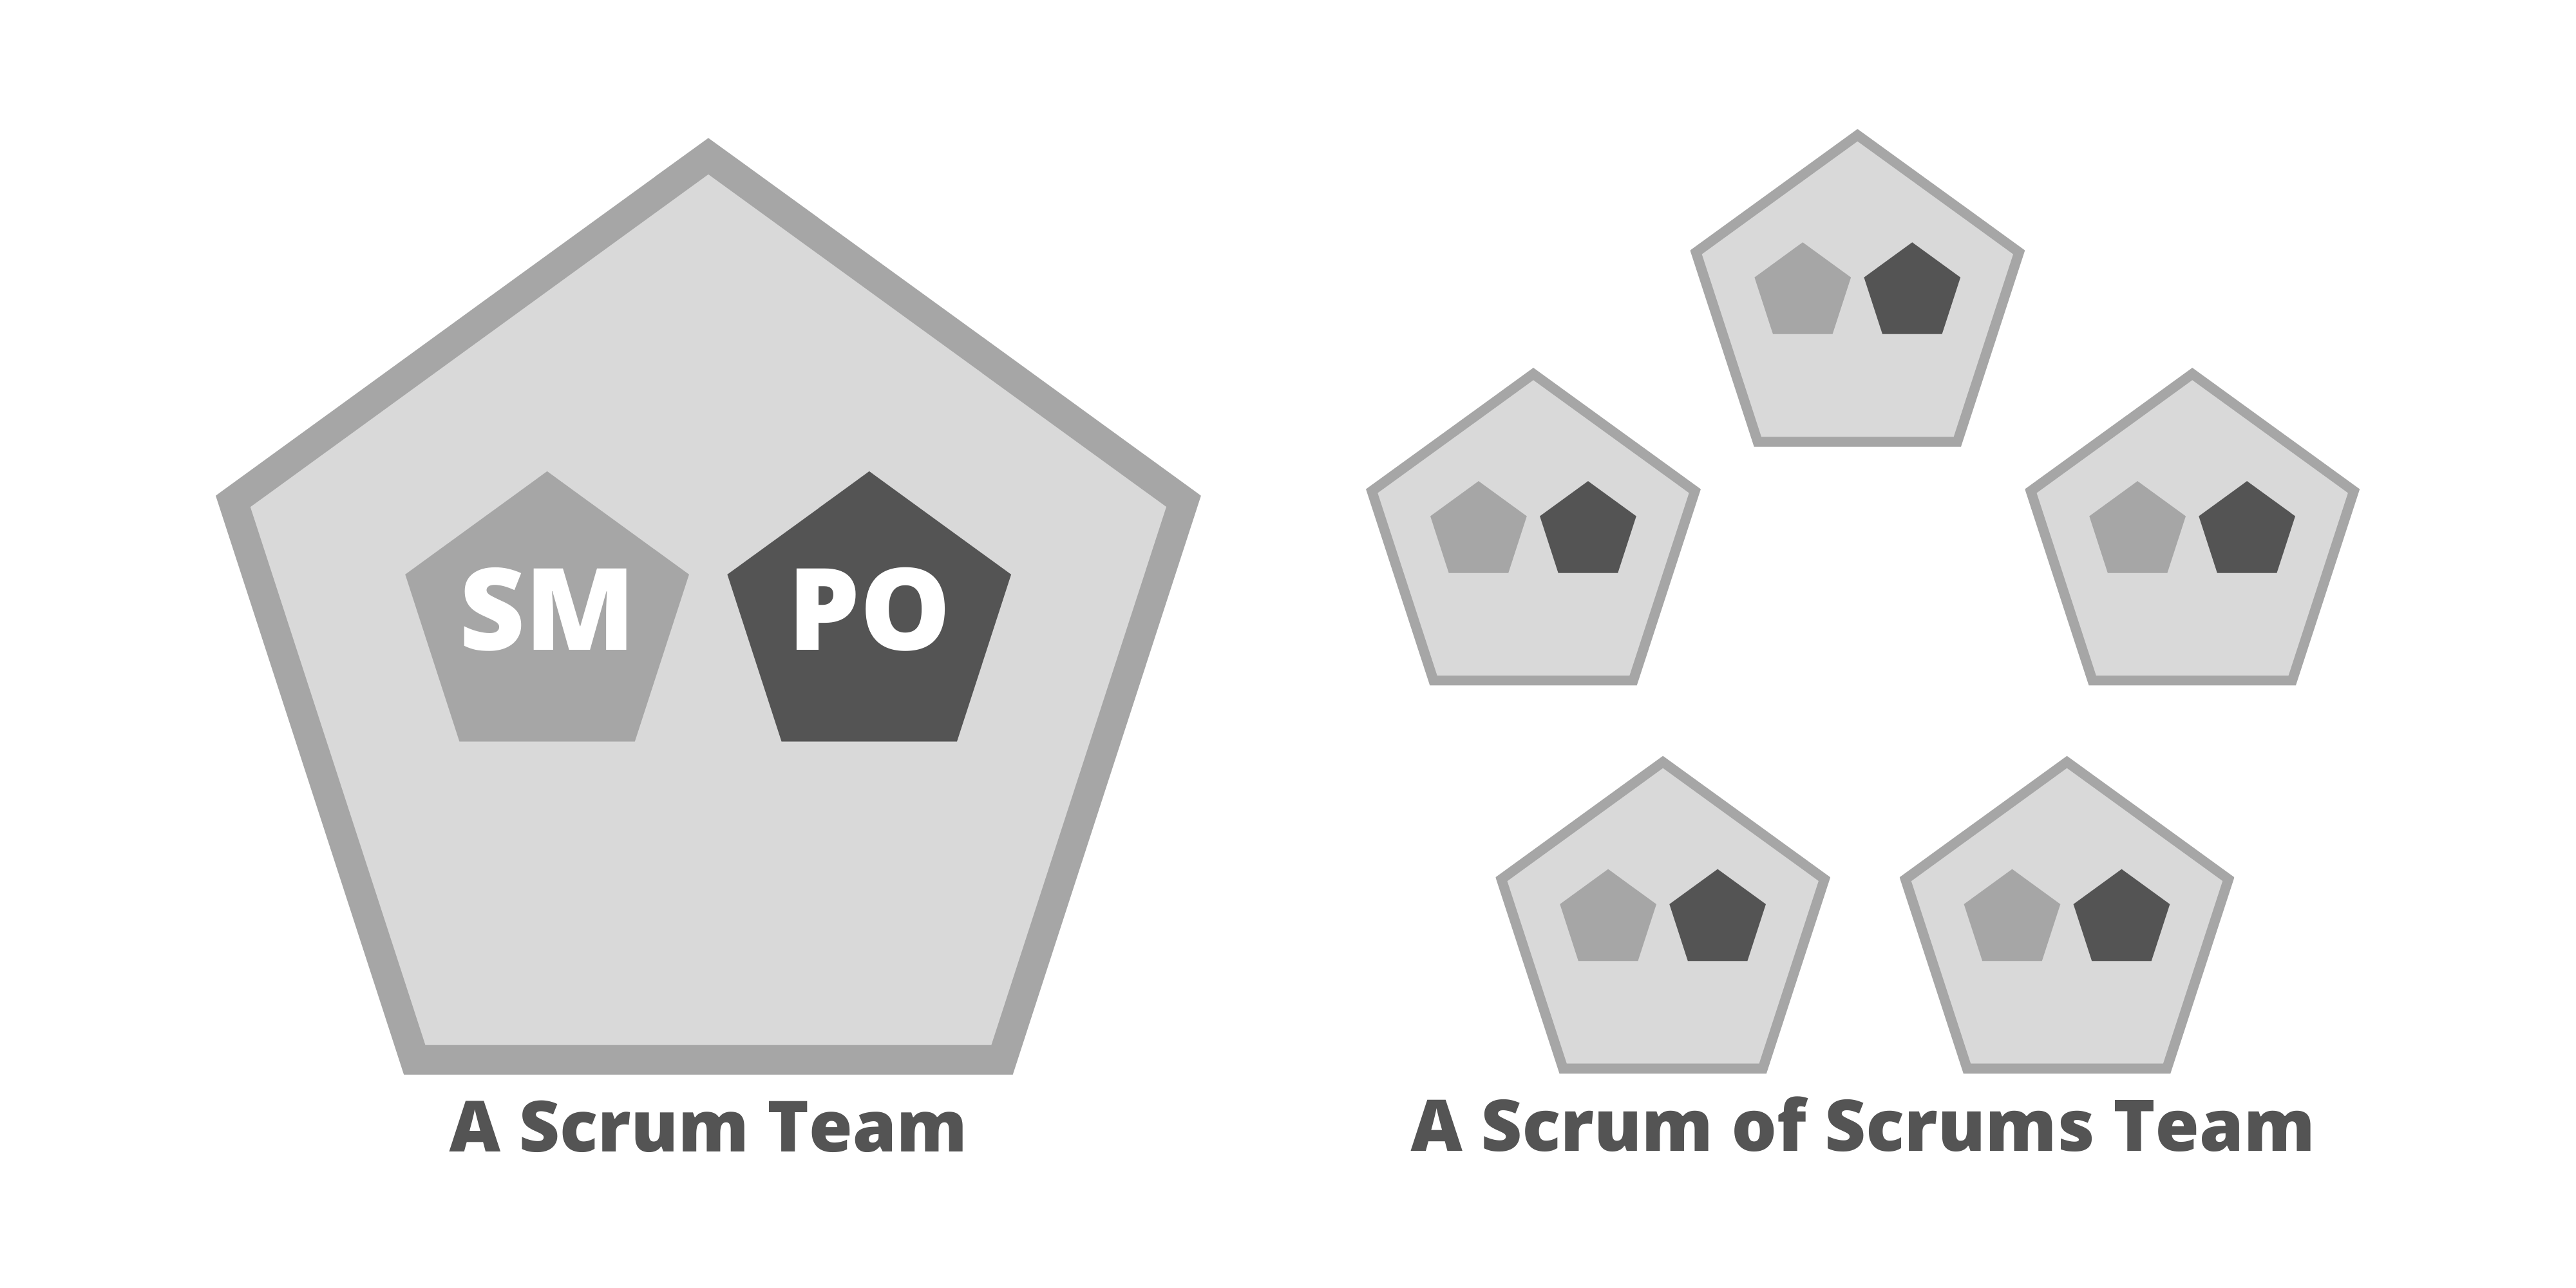
\includegraphics[scale=0.15]{1.png}
\end{figure}


\iffalse
\emph{
 NOTE: In the above and following diagrams, light-grey outlined pentagons represent a team. Where applicable, we have chosen to represent the SM \& PO as smaller pentagons. These diagrams are meant to be examples only, as each organizational diagram may differ greatly.}
\fi
注意: 上図およびこの後の図では、薄い灰色で囲まれた五角形がチームを表す。状況に応じて、SMとPOをこれより小さい五角形で表すことにした。組織図は組織によって大きく異なる可能性があるため、これらの図は例示のみを目的としている。

\iffalse
\subsubsection{Scaling in Larger
Organizations}\label{scaling-in-larger-organizations}
\fi
\subsubsection{大規模組織でのスケーリング}\label{scaling-in-larger-organizations}

\iffalse
Depending upon the size of an implementation, more than one Scrum of
Scrums may be needed to deliver a complex product. In such cases, a
Scrum of Scrum of Scrums (SoSoS) can be created out of multiple Scrums
of Scrums. Each of these will have scaled versions of each Scrum of
Scrums' roles, artifacts, and events.
\fi
実装の規模に応じて、複雑なプロダクトの提供には複数のスクラムオブスクラムが必要な場合がある。そのような場合には、複数のスクラムオブスクラムからスクラムオブスクラムオブスクラム(SoSoS)を編成できる。それぞれが、各スクラムオブスクラムからスケールされたそれ自身の役割、作成物、イベントを持つことになる。

\iffalse
Scaling the Scrum of Scrums reduces the number of communication pathways
within the organization so that complexity of communication overhead is
limited. The SoSoS interfaces with a Scrum of Scrums in the exact same
manner that a Scrum of Scrums interfaces with a single Scrum Team, which
allows for linear scalability.
\fi
スクラムオブスクラムをスケールすることで、組織内のコミュニケーション経路の数が削減されるので、コミュニケーションの経路の複雑さや、オーバーヘッドが軽減される。SoSoSは、スクラムオブスクラムが単一のスクラムチームとインタフェースするのとまったく同様の方法でスクラムオブスクラムとインタフェースするため、リニアなスケーラビリティが実現する。

\begin{figure}[H]
    \centering
    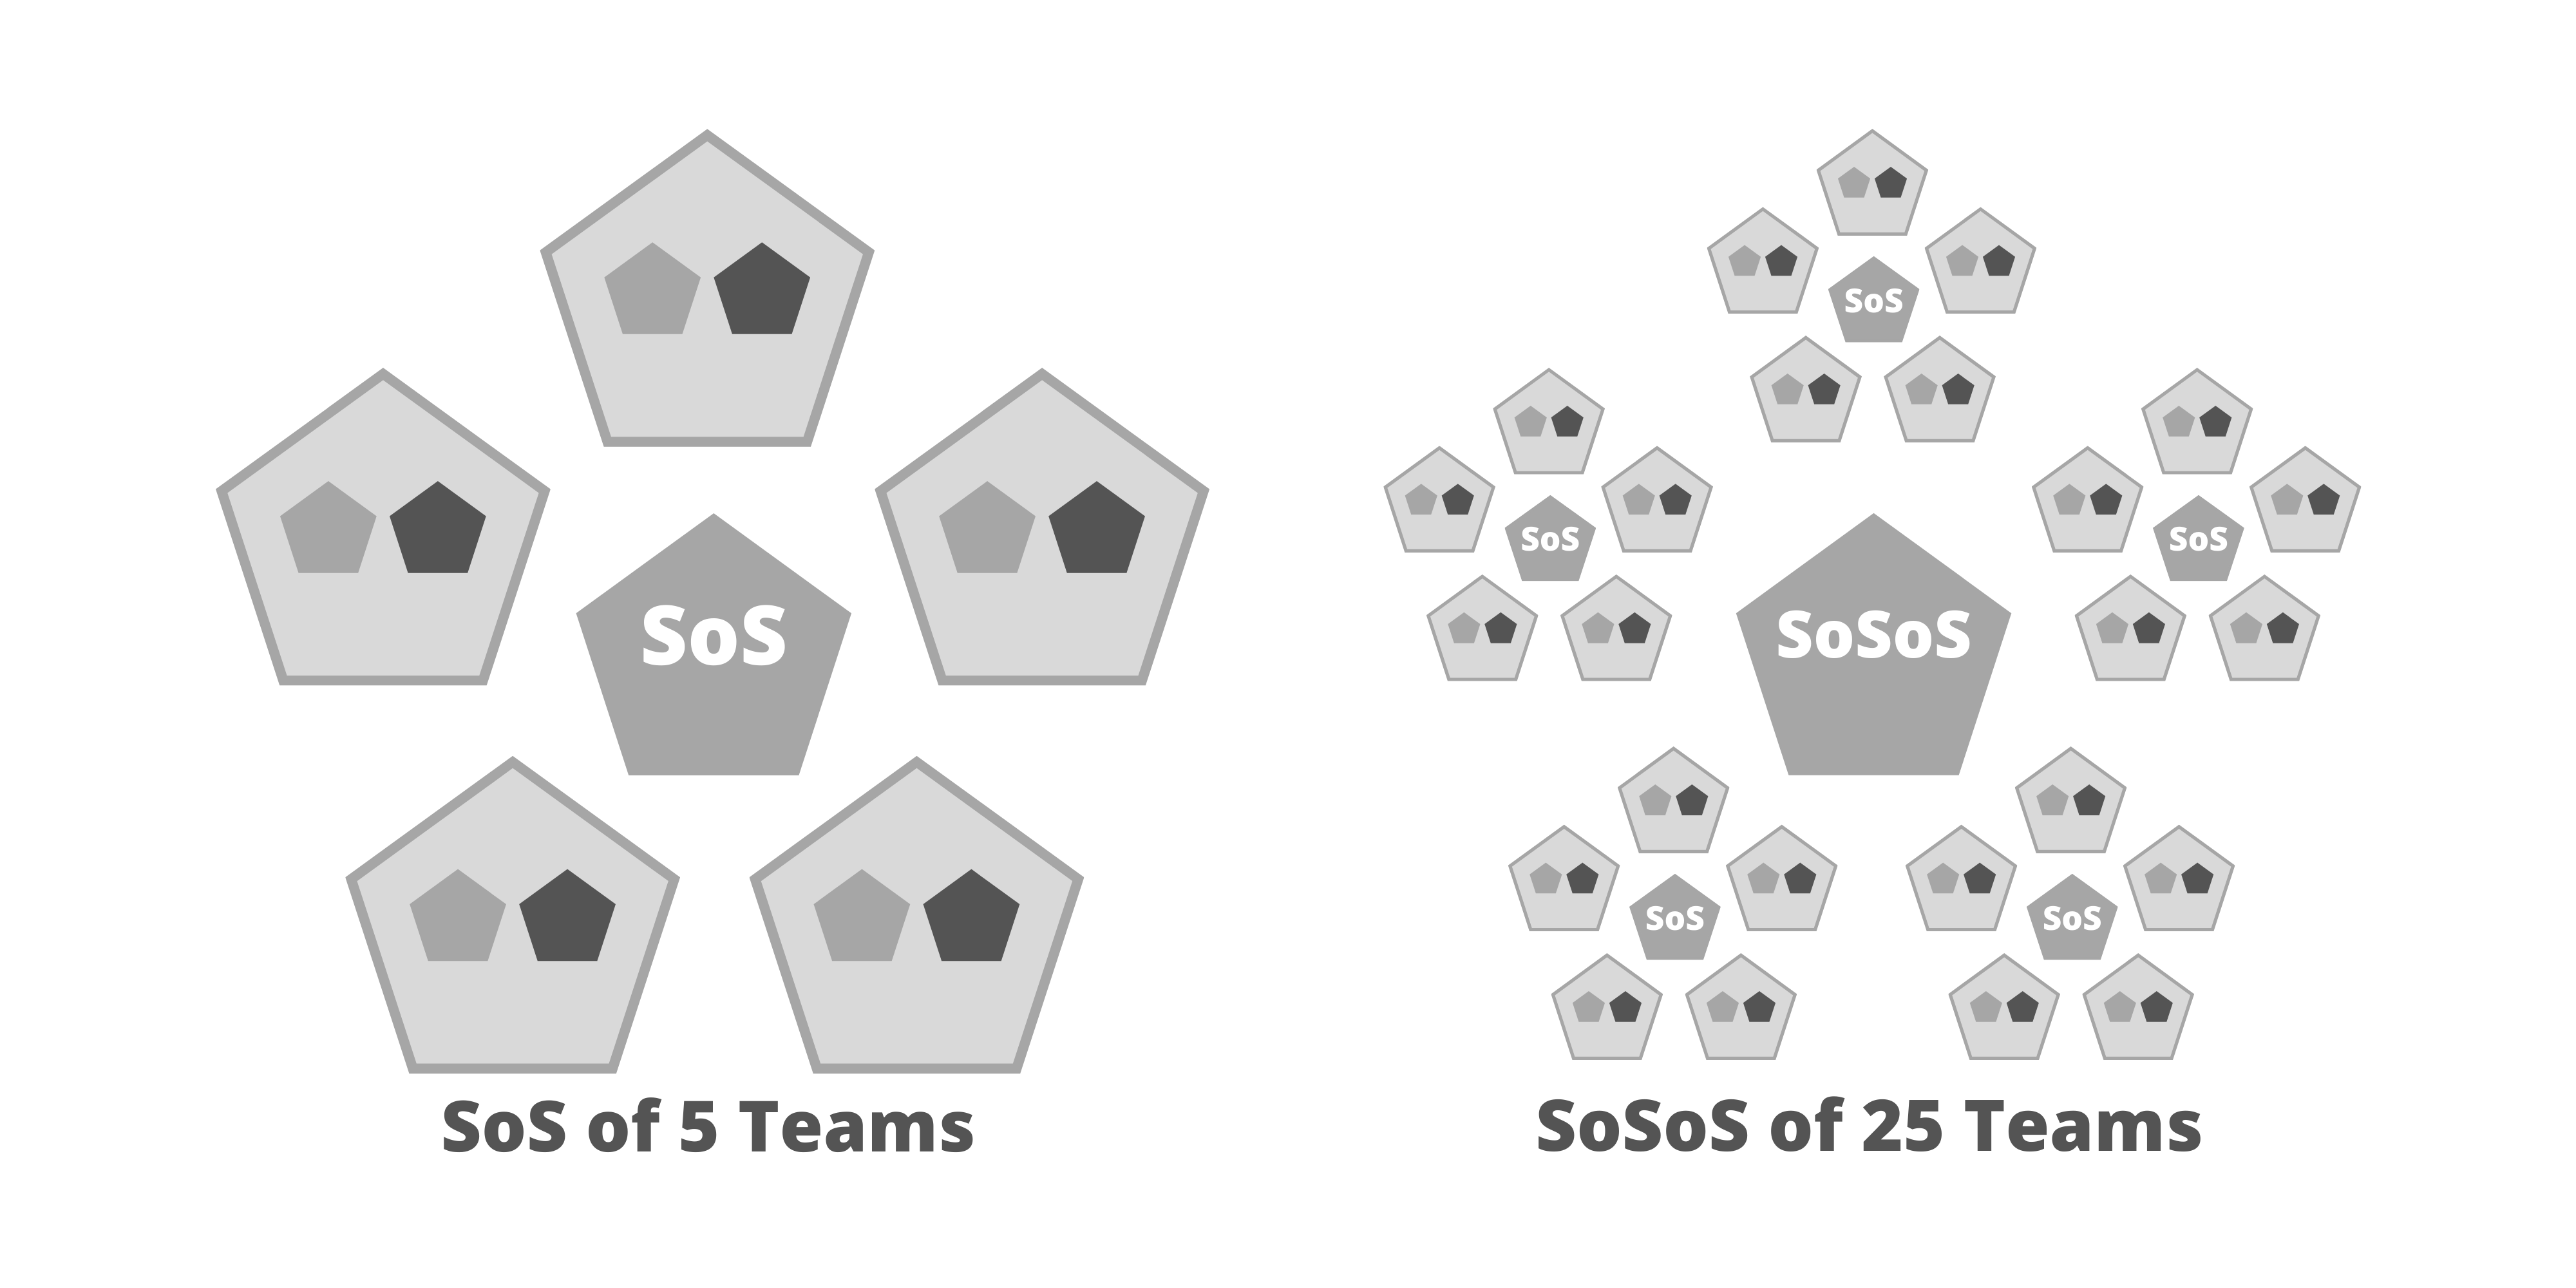
\includegraphics[scale=0.15]{2.png}
  
\end{figure}

\iffalse
\emph{NOTE: For simplicity, the numbers of teams and groupings in the
sample diagrams are symmetrical. They are meant to be examples only, as
each organizational diagram may differ greatly.}
\fi
注意: 簡潔にするために、例の図に含まれるチームとグループの数は対称的にしている。組織図は組織によって大きく異なる可能性があるため、これらの図は例示のみを目的としている。

\iffalse
\subsubsection{Scaling the Events and
Roles}\label{scaling-the-events-and-roles}
\fi
\subsubsection{イベントと役割のスケーリング}\label{scaling-the-events-and-roles}

\iffalse
If a Scrum of Scrums (SoS) operates as a Scrum Team, then it needs to scale the Scrum Events and the teams' corresponding accountabilities. To coordinate the ``how'' in every Sprint, a SoS will need to hold scaled versions of the Daily Scrum and Sprint Retrospective. To coordinate the ``what'' in every Sprint, a SoS will need to hold scaled versions of Sprint Planning and a Sprint Review. As an ongoing practice, Backlog Refinement will also need to be done at scale.
\fi
スクラムオブスクラム(SoS)がスクラムチームとして機能する場合は、スクラムイベントと、チームの対応する責任をスケールする必要がある。各スプリントの“How”を調整するために、SoSは、スケールされたデイリースクラムとスプリントレトロスペクティブを行う必要がある。各スプリントの“What”を調整するために、SoSは、スケールされたスプリントプランニングとスプリントレビューを行う必要がある。継続的な活動として、バックログリファインメントもスケールされる必要がある。

\iffalse
The scaled versions of the Daily Scrum and Retrospective are facilitated by a Scrum Master for the group, called the Scrum of Scrums Master (SoSM). The scaled versions of the Sprint Review and Backlog Refinement are facilitated by a Product Owner Team guided by a Chief Product Owner (CPO). The scaled version of Sprint Planning is held with the Product Owner Team and the Scrum Masters. The Product Owner Team gains insight into what will be delivered in the current Sprint and the Scrum Masters gain insight into capacity and technical capabilities. The roles of Scrum of Scrums Master and Chief Product Owner scale into the leadership groups which then drive their corresponding cycles, satisfying the components of Scrum@Scale.
\fi
スケールされたデイリースクラムとレトロスペクティブは、グループのスクラムマスター(スクラムオブスクラムマスター、SoSMと呼ばれる)がファシリテートする。スケールされたスプリントレビューとバックログリファインメントは、チーフプロダクトオーナー(CPO)が率いるプロダクトオーナーチームがファシリテートする。スケールされたスプリントプランニングは、プロダクトオーナーチームとスクラムマスターが行う。プロダクトオーナーチームは、現在のスプリントで何が提供されるかの洞察を得て、スクラムマスターは、キャパシティと技術的な能力の洞察を得る。スクラムオブスクラムマスターとチーフプロダクトオーナーの役割はリーダーシップグループにスケールされ、スクラムマスターサイクルとプロダクトオーナーサイクルをそれぞれ促進し、Scrum@Scaleのコンポーネントの要求を満たす。


\iffalse
\subsubsection{Event: The Scaled Daily Scrum
(SDS)}\label{event-the-scaled-daily-scrum}
\fi
\subsubsection{イベント: スケールドデイリースクラム(SDS)}\label{event-the-scaled-daily-scrum}

\iffalse
The main talking points of a Daily Scrum are the progress towards the Sprint Goal and impediments to meeting that commitment. In a scaled setting, the Scrum of Scrums needs to understand collective progress and be responsive to impediments raised by participating teams; therefore, at least one representative from each team attends a Scaled Daily Scrum (SDS). Any person or number of people from participating teams may attend as needed.
\fi
デイリースクラムの主なトピックは、スプリントゴールに向けた進捗と、確約(コミットメント)を果たすうえでの障害物である。スケールされた状況では、スクラムオブスクラムは、全体の進捗を理解し、参加チームが提起した障害物に対応する必要がある。よって、各チームから少なくとも1人の代表者がスケールドデイリースクラム(SDS)に参加する。必要に応じて、参加チームのだれでも、何人でも参加することができる。

\iffalse
To optimize collaboration and performance, the Scaled Daily Scrum event mirrors the Daily Scrum, in that it:
\fi
コラボレーションとパフォーマンスを最適化するために、スケールドデイリースクラムイベントは、以下の通り、デイリースクラムとまったく同じやり方で行う。


\begin{itemize}
\itemsep1pt\parskip0pt\parsep0pt
\iffalse
\item
  Is time-boxed to 15 minutes or less
\item
  Must be attended by a representative of each team.
\item
  Is a forum to discuss how teams can work together more effectively,
  what has been done, what will be done, what is going wrong \& why, and
  what the group is going to do about it
\fi
\item
15分以下のタイムボックス
\item
各チームの代表者が参加しなければならない
\item
チームが、どうすればチームが協力してより効果的に働けるか、何が完成したか、何をこれから完成するか、何が上手くいっていないかとその理由、それに関してグループがこれから何をするかを議論するフォーラム
\end{itemize}

\iffalse
Some examples of questions to be answered:
\fi
回答される質問の例は以下の通り。

\begin{itemize}
\itemsep1pt\parskip0pt\parsep0pt
\iffalse
\item
  What impediments does a team have that will prevent them from accomplishing their Sprint Goal or that will impact the planned delivery?
\item
  Is a team doing anything that will prevent another team from accomplishing their Sprint Goal or that will impact their planned delivery?
\item
 Have any new dependencies between the teams or a way to resolve an existing dependency been discovered?
\fi
\item
チームのスプリントゴールの達成を妨げる、あるいはデリバリー計画に影響を与える障害物は何か?
\item
チームは、他のチームのスプリントゴールの達成を妨げる、あるいはデリバリー計画に影響を与えることをしているか?
\item
チーム間の新たな依存関係を発見したか、または既存の依存関係を解決する方法を発見したか?
\end{itemize}

\iffalse
\subsubsection{Event: The Scaled
Retrospective}\label{event-the-scaled-retrospective}
\fi
\subsubsection{イベント: スケールドレトロスペクティブ}\label{event-the-scaled-retrospective}

\iffalse
Every Sprint, the Scrum of Scrums holds a scaled version of the Sprint Retrospective where the Scrum Masters of each team get together and discuss what experiments have been done to drive continuous improvement and their results. Additionally, they should discuss the next round of experiments and how successful improvements can be leveraged across the group of teams or beyond.
\fi
スプリントごとに、スクラムオブスクラムは、スケールされたスプリントレトロスペクティブを行う。このレトロスペクティブでは、各チームのスクラムマスターが集まり、継続的な改善を促すために行った実験とその結果を話し合う。さらに、次回の実験や、成功した改善をチームのグループ全体、あるいはそれ以外にも活用できる方法も話し合うべきである。


\iffalse
\subsection{The Scrum Master Cycle: Coordinating the
``How''}\label{the-scrum-master-cycle}
\fi
\subsection{スクラムマスターサイクル: “How”を調整する}\label{the-scrum-master-cycle}

\iffalse
\subsubsection{Role: The Scrum of Scrums Master
(SoSM)}\label{role-the-scrum-of-scrums-master}
\fi
\subsubsection{役割: スクラムオブスクラムマスター(SoSM)}\label{role-the-scrum-of-scrums-master}

\iffalse
The Scrum Master of the Scrum of Scrums is called the Scrum of Scrums Master (SoSM). The Scrum of Scrums Master is accountable for ensuring the Scaled events take place, are productive, positive, and kept within the time-box. The Scrum of Scrums Master may be one of the team's Scrum Masters or a person specifically dedicated to this role. They are accountable for the release of the joint teams' efforts and continuously improving the effectiveness of the Scrum of Scrums. This includes greater team throughput, lower cost, and higher quality. In order to achieve these goals, they must:
\fi
スクラムオブスクラムのスクラムマスターをスクラムオブスクラムマスター(SoSM)と呼ぶ。スクラムオブスクラムマスターは、スケールされたイベントが確実に行われ、生産的でポジティブであり、タイムボックスが守られるようにする責任を負う。スクラムオブスクラムマスターは、チームのスクラムマスターがなる場合もあれば、この役割に特化した個人の場合もある。SoSMは、共同チームの努力の結果であるプロダクトのリリースと、スクラムオブスクラムの有効性を継続的に改善する責任を負う。これには、チームのスループットの向上、コストの削減、品質の向上が含まれる。これらのゴールを達成するために、SoSMは次のようにしなければならない。

\begin{itemize}
\itemsep1pt\parskip0pt\parsep0pt
\iffalse
\item
  Work closely with the Chief Product Owner to deliver a potentially
  releasable product increment at least every Sprint
\item
  Coordinate the teams' delivery with the Product Owners Team's release
  plans
\item
  Make impediments, process improvements, and progress visible to the
  organization
\item
  Facilitate the prioritization and removal of impediments, paying
  particular attention to cross-team dependencies
\fi
\item
チーフプロダクトオーナーと緊密に連携し、少なくとも各スプリントでリリース判断可能なプロダクトインクリメントを届ける
\item
チームのデリバリーをプロダクトオーナーチームのリリースプランに応じて調整する
\item
組織に対して障害物、プロセス改善、進捗を見える化する
\item
チーム横断的な依存関係に特に注意を払いつつ、障害物の優先順位付けと除去を促す
\end{itemize}

\iffalse
The Scrum of Scrums Master is a true leader who serves the teams and the organization by understanding cross-team dependencies, including those outside of the Scrum of Scrums and enabling cross-team coordination and communication. They are accountable for keeping the Chief Product Owner, stakeholders, and larger organization informed by radiating information about product development progress, impediments removal status, and other metrics. The Scrum of Scrums Master leads by example, mentoring others to increase the effectiveness and adoption of Scrum throughout the organization.
\fi
スクラムオブスクラムマスターは、チームと組織に奉仕する真のリーダーであり、スクラムオブスクラムの外部も含めて、チーム横断的な依存関係を理解し、チーム横断的な調整とコミュニケーションを可能にする。SoSMは、プロダクト開発の進捗、障害物の除去状況、その他のメトリクスの情報を発信することで、チーフプロダクトオーナー、ステークホルダーさらには組織全体に情報を提供し続けることに責任を負う。スクラムオブスクラムマスターは、組織全体でスクラムの有効性と導入を高めるよう他者をメンタリングすることなどで、リーダーシップを発揮する。

\iffalse
In the case where multiple Scrum of Scrums are grouped into a Scrum of Scrum of Scrums, then a Scrum of Scrum of Scrums Master (SoSoSM) is needed to coordinate from that wider perspective.
\fi
複数のスクラムオブスクラムが1つのスクラムオブスクラムオブスクラムにグループ化された場合、より広い観点から調整を行うために、スクラムオブスクラムオブスクラムマスター(SoSoSM)が必要になる。


\iffalse
\subsubsection{The Hub of the SM Cycle: The Executive Action Team
(EAT)}\label{the-hub-of-the-sm-cycle}
\fi
\subsubsection{SMサイクルのハブ: エグゼクティブアクションチーム(EAT)}\label{the-hub-of-the-sm-cycle}

\iffalse
The Executive Action Team (EAT) fulfills the Scrum Master accountabilities for an entire agile organization. This leadership team creates an agile ecosystem that allows the Reference Model to function optimally, by:
\fi
エグゼクティブアクションチーム(EAT)は、アジャイル組織全体に対してスクラムマスターの責任を果たす。このリーダーシップチームは、以下を行うことで、リファレンスモデルが最適に機能するアジャイルエコシステムを生み出す。

\begin{itemize}
\itemsep1pt\parskip0pt\parsep0pt
\iffalse
\item
  implementing the Scrum values
\item
  assuring that Scrum roles are created and supported
\item
  Scrum events are held and attended
\item
 Scrum Artifacts and their associated commitments are generated, made transparent, and updated throughout each Sprint.
\item
 formulating guidelines and procedures that act as a translation layer between the Reference model and any part of the organization that is not agile.
\fi
\item
スクラムの価値基準を導入する
\item
スクラムの役割が確実に作成・支援されるようにする
\item
スクラムイベントが実施・出席されるようにする
\item
各スプリントで、スクラムの作成物とそれに関連する確約(コミットメント)が作り出され、透明性が保たれ、各スプリントで更新されるようにする
\item
リファレンスモデルと組織内の非アジャイル部分との間の変換層として機能するガイドラインと手続きを策定する
\end{itemize}

\iffalse
The Executive Action Team is accountable for removing impediments that cannot be removed by members of the Scrum of Scrums (or wider network). Therefore, it must be comprised of individuals who are empowered, politically and financially, to remove them. The function of the Executive Action Team is to coordinate multiple Scrums of Scrums (or wider networks) and to interface with any non-agile parts of the organization. As with any Scrum Team, it needs a Product Owner, a Scrum Master, and a transparent backlog.
\fi
エグゼクティブアクションチームは、スクラムオブスクラム(または、より広範なネットワーク)のメンバーで取り除くことができない障害物を除去する責任を負う。したがって、それを除去するために政治的、財務的に権限を与えられた個人で構成されなければならない。エグゼクティブアクションチームの機能は、複数のスクラムオブスクラム(または、より広範なネットワーク)を調整することと、組織内の非アジャイル部分とインタフェースすることである。スクラムチームと同様に、プロダクトオーナー、スクラムマスター、透明性のあるバックログが必要である。

\begin{figure}[H]
    \centering
    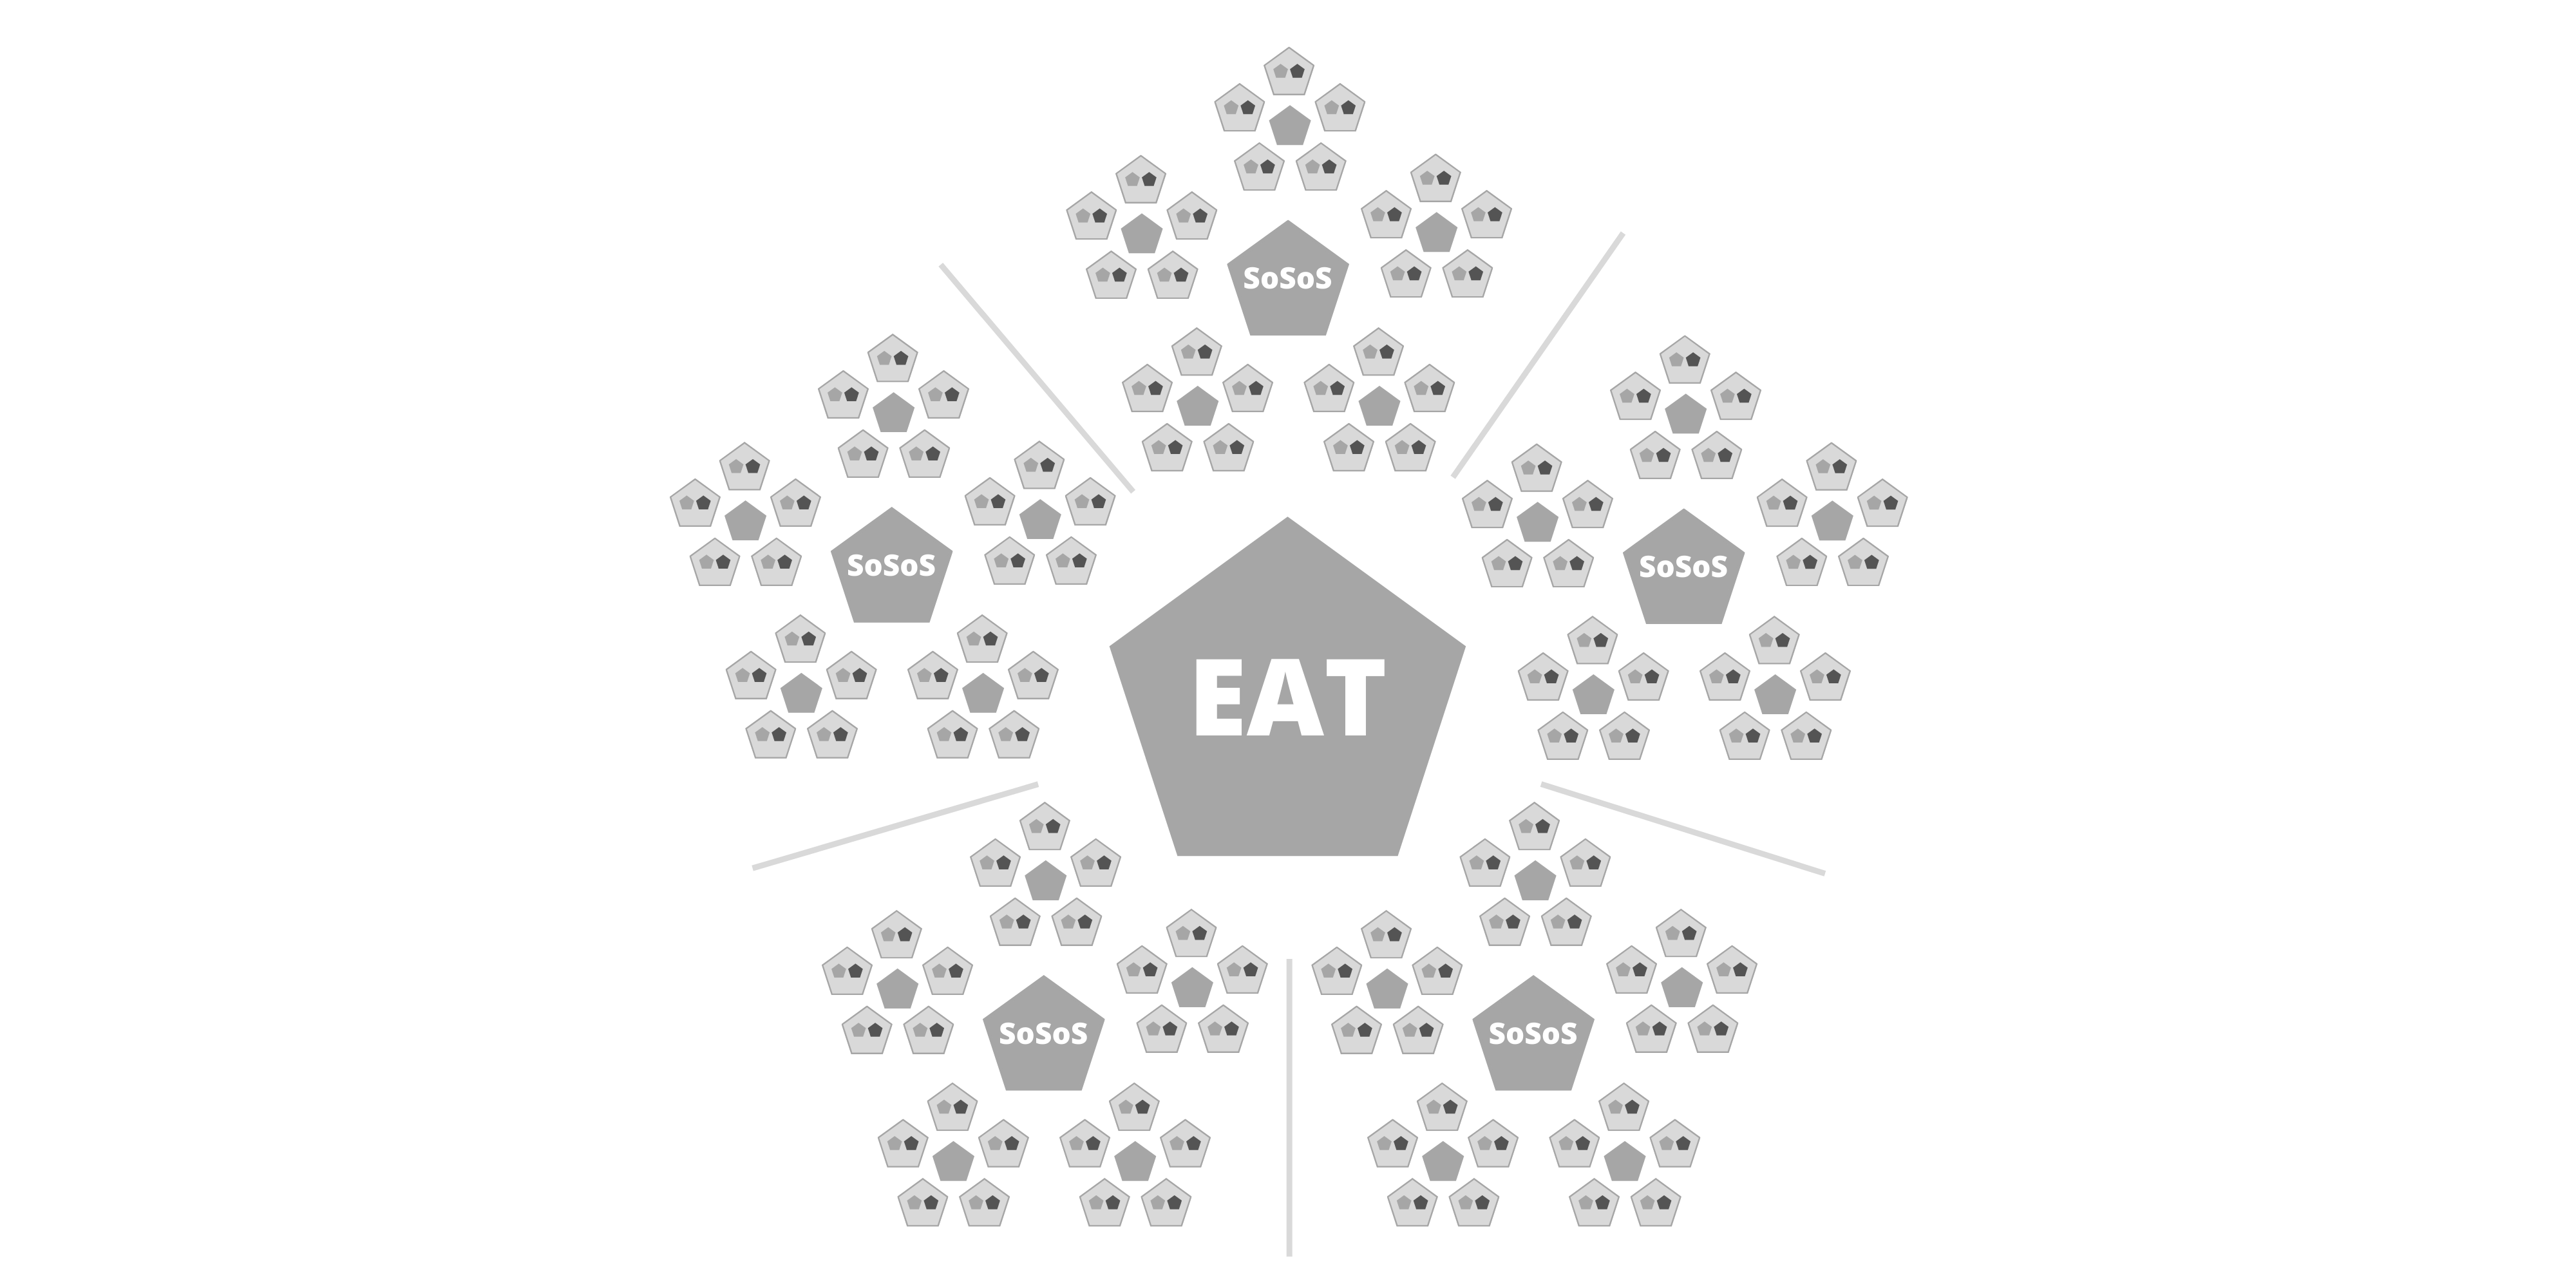
\includegraphics[scale=0.15]{3.png}
    
\end{figure}


\iffalse
\emph{Sample Diagram showing an EAT coordinating 5 groupings of 25
teams}
\fi
25チームの5つのグループを調整するEATを示す参考図

\iffalse
\subsubsection{EAT Backlog and
Responsibilities}\label{EAT-backlog-and-responsibilities}
\fi
\subsubsection{EATのバックログと責務}\label{EAT-backlog-and-responsibilities}

\iffalse
The product of the Executive Action Team (EAT) is the creation of an Agile operating system for the organization. The EAT curates a Product Backlog consisting of initiatives for the ongoing transformation of the organization to achieve the goal of greater business agility. This backlog also includes process improvements which remove impediments and ones that need to be standardized.
\fi
エグゼクティブアクションチーム(EAT)の成果は、組織のアジャイルオペレーティングシステムの構築である。EATは、ビジネスアジリティの向上という目標を達成するために、組織の継続的な変革に向けた取り組みをプロダクトバックログとして整理選択し、提示する。このバックログには、障害物を除去するプロセス改善と、標準化が必要なプロセス改善も含まれる。

\iffalse
The Executive Action Team's responsibilities include, but are not
limited to:
\fi
エグゼクティブアクションチームの責務には以下を含まれるが、これらに限定されない。

\begin{itemize}
\itemsep1pt\parskip0pt\parsep0pt
\iffalse
\item
  Creating an agile operating system for the Reference Model as it scales through an organization, including corporate operational rules, procedures, and guidelines to enable agility
\item
 Ensuring a Product Owner organization is created, funded, and supported
\item
  Measuring and improving the quality of Scrum in an organization
\item
  Building capability within an organization for business agility
\item
  Creating a center for continuous learning for Scrum professionals
\item
  Supporting the exploration of new ways of working
\fi
\item
組織でスケール可能なリファレンスモデルのためのアジャイルオペレーティングシステムを作成する(アジリティを得るための企業の運営ルール、手続き、ガイドラインを含む)
\item
プロダクトオーナー組織が作成され、資金提供され、支援されることを保証する
\item
組織でスクラムの品質を測定し改善する
\item
ビジネスアジリティ実現に向けた組織内の能力を構築する
\item
スクラムのプロフェッショナルのための継続的学習の拠点を作る
\item
新しい働き方の探求を支援する
\end{itemize}

\iffalse
The function of the Executive Action Team is to see that this backlog is carried out. They may do this themselves or empower another group to do it. As the Executive Action Team is accountable for the quality of Scrum within the organization, the entire Scrum Master organization reports into them.
\fi
エグゼクティブアクションチームの役割は、このバックログが実行されていることを確認することである。これをEAT自体で行うことも、別のグループに権限を与えて行わせることもできる。エグゼクティブアクションチームは組織内のスクラムの品質に責任を負うため、スクラムマスター組織全体がEATに報告する。

\iffalse
The Scrum Master organization (Scrum Masters, Scrum of Scrum Masters, and the Executive Action Team) work as a whole to implement the Scrum Master Cycle components. These unique components are:
\fi
スクラムマスター組織(スクラムマスター、スクラムオブスクラムマスター、エグゼクティブアクションチーム)は、スクラムマスターサイクルのコンポーネントを実装するために全体として機能する。固有のコンポーネントは以下の通り。


\begin{itemize}
\itemsep1pt\parskip0pt\parsep0pt
\iffalse
\item
  Continuous Improvement and Impediment Removal
\item
  Cross-Team Coordination
\item
  Delivery
\fi
\item
継続的改善と障害物の除去
\item
チーム横断の調整
\item
デリバリー
\end{itemize}

\iffalse
\subsubsection{Continuous Improvement and Impediment
Removal}\label{Continuous-improvement-and-impediment-removal}
\fi
\subsubsection{継続的改善と障害物除去}\label{Continuous-improvement-and-impediment-removal}

\iffalse
Ideally, impediments should be removed as quickly as possible. This is critical to avoid scaling the impediments themselves, and because unresolved impediments may slow productivity. Therefore, the goals of Continuous Improvement and Impediment Removal are to:
\fi
障害物の除去は、できる限り迅速に除去されるのが理想的である。これは、障害物自体が組織に拡散することを回避し、未解決の障害物によって生産性を低下させないために不可欠である。よって、継続的改善と障害物の除去のゴールは以下の通り。


\begin{itemize}
\itemsep1pt\parskip0pt\parsep0pt
\iffalse
\item
  identify impediments and reframe them as opportunities to improve
\item
  ensure transparency and visibility in the organization to effect
  change
\item
  maintain an effective environment for prioritizing and removing
  impediments
\item
  verify that improvements have positively impacted team and/or product
  metrics
\fi
\item
障害物を特定し、改善の機会としてそれを捉え直す
\item
変化を可能にする透明性と可視性を組織内に確保する
\item
障害物の優先順位付けと除去に効果的な環境を維持する
\item
改善がチーム/プロダクトのメトリクスにプラスの影響を与えていることを確認する
\end{itemize}

\iffalse
\subsubsection{Cross-Team Coordination}\label{cross-team-coordination}
\fi
\subsubsection{チーム横断の調整}\label{cross-team-coordination}

\iffalse
When multiple teams are needed for the creation of a shared product,
streamlined collaboration is required for success. Therefore, the goals
of Cross-Team Coordination are to:
\fi
共通のプロダクトの作成に複数のチームが必要な場合、成功するにはコラボレーションの合理化が必要である。よって、チーム横断の調整のゴールは以下の通り。

\begin{itemize}
\itemsep1pt\parskip0pt\parsep0pt
\iffalse
\item
  sync up similar processes across multiple related teams
\item
  mitigate cross-team dependencies to ensure they do not become
  impediments
\item
  maintain alignment of team norms and guidelines for consistent output
\fi
\item
関連する複数のチーム間で類似のプロセスを同期させる
\item
チーム間の依存関係を緩和し、障害物とならないようにする
\item
一貫性のあるアウトプットのために、チームの規範とガイドラインの整合性を維持する
\end{itemize}

\iffalse
\subsubsection{Delivery}\label{Delivery}
\fi
\subsubsection{デリバリー}\label{Delivery}

\iffalse
Since the goal of the Scrum of Scrums is to function as a single unit and release together, how the product is delivered falls under their scope as a group. The Product Owner Team determines both the content of the release and the optimal time to deliver the increment to customers.  Therefore, the goals of Delivery for the Scrum of Scrums are to:
\fi
スクラムオブスクラムのゴールは、単一のユニットとして機能し、一緒にリリースすることなので、プロダクトをどのようにデリバリーするかは、スクラムオブスクラムのグループとしての範囲に含まれる。プロダクトオーナーチームは、リリースの内容と、インクリメントを顧客に届ける最適なタイミングの両方を決定する。よって、スクラムオブスクラムのデリバリーのゴールは以下の通り。

\begin{itemize}
\itemsep1pt\parskip0pt\parsep0pt
\iffalse
\item
  deliver a consistent flow of valuable finished product to customers
\item
  integrate the work of different teams into one seamless product
\item
  ensure a high-quality customer experience
\fi
\item
顧客に一貫した流れで価値ある完成したプロダクトを届ける
\item
異なるチームの作業をシームレスな1つのプロダクトに統合する
\item
高品質な顧客体験を確保する
\end{itemize}

\iffalse
\subsection{The Product Owner Cycle: Coordinating the
``What''}\label{The-product-owner-cycle}
\fi
\subsection{プロダクトオーナーサイクル: “What”を調整する}\label{The-product-owner-cycle}


\iffalse
\subsubsection{Scaling the Product Owner - The Product Owner
Cycle}\label{Scaling-the-product-owner}
\fi
\subsubsection{プロダクトオーナーのスケーリング - プロダクトオーナーサイクル}\label{Scaling-the-product-owner}


\iffalse
For each Scrum of Scrums, there is a shared common backlog that feeds the network of teams. It requires a Product Owner Team (PO Team), including a Chief Product Owner, who is accountable as the Product Owner for the group of teams. The PO Team's main focus is ensuring that the individual teams' priorities follow along a single path. This allows them to coordinate their individual team's backlogs and build alignment with stakeholders and customer needs.
\fi
スクラムオブスクラムごとに、チームのネットワークに供給する共通のバックログがある。そして、スクラムオブスクラムのプロダクトオーナーとして責任を負う、チーフプロダクトオーナーを含むプロダクトオーナーチーム(POチーム)が必要である。POチームが主に重視するのは、個々のチームの優先順位を一列に並べることである。これによって、個々のチームのバックログの調整と、ステークホルダーと顧客ニーズの整合性の確立が可能になる。


\iffalse
Each team's Product Owner is accountable for the composition and prioritization of their team's Sprint backlog and may pull items from the common backlog or generate independent backlog items at their discretion as needed to meet business objectives.
\fi
各チームのプロダクトオーナーは、自チームのスプリントバックログの構成と優先順位付けに責任を持ち、ビジネス目標の達成に必要な場合は、自身の裁量で、共通バックログからアイテムを引き出したり、独立したバックログアイテムを生成することができる。

\iffalse
The main functions of the Product Owner Team are to:
\fi
プロダクトオーナーチームの主な役割は以下の通り。

\begin{itemize}
\itemsep1pt\parskip0pt\parsep0pt
\iffalse
\item
  communicate the overarching vision for the product \& make it visible
  to everyone in the organization
\item
  build alignment with key stakeholders to secure support for backlog
  implementation
\item
  generate a single, prioritized backlog; ensuring that duplication of
  work is avoided
\item
  work with the Scrum of Scrums Master to create a minimally uniform
  ``Definition of Done'' that applies to all team
\item
  eliminate dependencies raised by the teams
\item
  generate a coordinated Roadmap and Release Plan
\item
  monitor metrics that give insight into the product and the market
\fi
\item
プロダクトの包括的なビジョンを伝達し、組織内の全員に見える化する
\item
主要なステークホルダーとの連携を構築し、バックログの実行に対する支援を確保する
\item
単一の優先順位付けされたバックログを生成し、チーム間の作業の重複を回避する
\item
スクラムオブスクラムマスターと協力して、全チームに適用される最小限で統一的な「完成の定義」を作成する
\item
チームが提起した依存関係を排除する
\item
調整されたロードマップとリリースプランを生成する
\item
プロダクトと市場に関する洞察力をもたらすメトリクスを測定する
\end{itemize}

\iffalse
\subsubsection{Role: The Chief Product Owner
(CPO)}\label{role-the-chief-product-owner}
\fi
\subsubsection{役割: チーフプロダクトオーナー(CPO)}\label{role-the-chief-product-owner}

\iffalse
The Chief Product Owner coordinates priorities with the Product Owner Team. Together they align backlog priorities with stakeholder and customer needs. The CPO may be an individual team Product Owner who plays this role as well, or they may be a person specifically dedicated to it. Their main responsibilities are the same as a regular Product Owner's now scaled:
\fi
チーフプロダクトオーナーは、プロダクトオーナーチームと一緒に優先順位を調整する。共同でバックログの優先順位をステークホルダーと顧客のニーズに合わせる。CPOは、この役割を兼任する個別チームのプロダクトオーナーである場合もあれば、この役割に専任した個人の場合もある。主な責務は通常のプロダクトオーナーと同じであるが、スケールされて以下のようになる。

\begin{itemize}
\itemsep1pt\parskip0pt\parsep0pt
\iffalse
\item
  Setting a strategic vision for the whole product
\item
  Creating a single, prioritized backlog to be delivered by all of the
  teams
\item
  Decide which metrics the Product Owner Team will monitor
\item
  Assess customer product feedback and adjust the common backlog
  accordingly
\item
  Facilitate the MetaScrum event (see below)
\fi
\item
プロダクト全体の戦略的ビジョンを設定する
\item
全チームに配布される、優先順位付けされた単一のバックログを作成する
\item
プロダクトオーナーチームが測定するメトリクスを決定する
\item
顧客からのプロダクトのフィードバックを評価し、それに応じて共通バックログを調整する
\item
メタスクラムイベント(以下参照)をファシリテートする
\end{itemize}

\iffalse
The Chief Product Owner is accountable along with their associated Scrum
of Scrums Masters for the efficient delivery of product increments
according to the Release Plan.
\fi
チーフプロダクトオーナーは、関連するスクラムオブスクラムマスターとともに、リリースプランに従ったプロダクトインクリメントの効率的なデリバリーに責任を負う。

\iffalse
\subsubsection{Scaling the Product Owner
Team}\label{scaling-the-product-owner-team}
\fi
\subsubsection{プロダクトオーナーチームのスケーリング}\label{scaling-the-product-owner-team}

\iffalse
Having Product Owner Teams enables a network design of Product Owners which scales along with their associated Scrum of Scrums. There is no specific term associated with these expanded units, nor do the Chief Product Owners of them have specific expanded titles. Each organization is encouraged to develop their own.
\fi
プロダクトオーナーチームを設けることで、関連するスクラムオブスクラムとともにスケールするプロダクトオーナーのネットワークデザインが可能になる。これらの拡張ユニットには特定の用語はなく、チーフプロダクトオーナーの特定の拡張された肩書もない。プロダクトオーナーチームやチーフプロダクトオーナー向けの用語や肩書は、各組織で独自に設定することを奨励する。

\iffalse
\subsubsection{The Hub of the PO Cycle: The Executive MetaScrum
(EMS)}\label{the-hub-of-the-po-cycle}
\fi
\subsubsection{POサイクルのハブ: エグゼクティブメタスクラム(EMS)}\label{the-hub-of-the-po-cycle}

\iffalse
To fulfill the Product Owner role for the entire agile organization, the
Chief Product Owners meet with executives and key stakeholders at an
Executive MetaScrum event. This event is derived from the MetaScrum
pattern\textsuperscript{\hyperref[citation5]{5}}. It is \emph{the forum}
for Leadership and other stakeholders to express their preferences to
the PO Team, negotiate priorities, alter budgets, or realign teams to
maximize the delivery of value. At no other time during the Sprint
should these decisions be made.
\fi
アジャイル組織全体に対してプロダクトオーナーの役割を果たすために、チーフプロダクトオーナーは、エグゼクティブメタスクラムイベントでエグゼクティブや主要なステークホルダーと会合する。

このイベントは、メタスクラムパターン\textsuperscript{\hyperref[citation5]{5}}.から派生している。これは、リーダーシップとその他のステークホルダーが、自らの好みをPOチームに伝え、優先順位を交渉し、予算を変更し、チームを再編成して価値の提供を最大化するためのフォーラムである。スプリント中の他のタイミングでは、こうした決定を行うべきではない。

\iffalse
At the Executive MetaScrum a dynamic group of leaders sets the
organizational vision and the strategic priorities, aligning all of the
teams around common goals.~ In order to be effective, the Chief Product
Owner facilitates and each team's Product Owner (or a proxy) must
attend. This event occurs as often as needed- at least once per Sprint-
to ensure an aligned backlog within the Scrum of Scrums.~ Optimally,
this group of leaders operates as a scrum team.
\fi
エグゼクティブメタスクラムでは、リーダーの動的グループが、組織のビジョンと戦略的な優先順位を設定し、共通のゴールに沿って全チームの方向性を揃える。効果的に行うために、チーフプロダクトオーナーがファシリテートし、各チームのプロダクトオーナー(またはその代理)が出席しなければならない。このイベントは、スクラムオブスクラム内でバックログの方向性を揃えるために、必要な頻度で行う(少なくとも各スプリントで1回)。理想は、このリーダーのグループがスクラムチームとして活動することである。

\iffalse
In the case of larger implementations where there are multiple Scrum of
Scrums, there may be multiple MetaScrums which have their strategic
backlog created and prioritized at an Executive MetaScrum.
\fi
複数のスクラムオブスクラムが存在する大規模な実装の場合、エグゼクティブメタスクラムで戦略的バックログの作成と優先順位付けがされた、複数のメタスクラムが存在する可能性がある。

\iffalse
\subsubsection{Coordinating the ``What'' - The Product Owner
Cycle}\label{coordinating-the-what}
\fi
\subsubsection{“What”を調整する - プロダクトオーナーサイクル}\label{coordinating-the-what}

\iffalse
The Product Owner organization (the Product Owners, the Chief Product
Owners, and the Executive MetaScrum) work as a whole to satisfy the
unique components of the Product Owner Cycle:
\fi
プロダクトオーナー組織(プロダクトオーナー、チーフプロダクトオーナー、エグゼクティブメタスクラム)は、プロダクトオーナーサイクルの以下の固有コンポーネントの要求を満たすために全体として機能する。

\begin{itemize}
\itemsep1pt\parskip0pt\parsep0pt
\iffalse
\item
  Strategic Vision
\item
  Backlog Prioritization
\item
  Backlog Decomposition \& Refinement
\item
  Release Planning
\fi
\item
戦略的ビジョン
\item
バックログの優先順位付け
\item
バックログの分割とリファインメント
\item
リリースプランニング
\end{itemize}

\iffalse
\subsubsection{Strategic Vision}\label{strategic-vision}
\fi
\subsubsection{戦略的ビジョン}\label{strategic-vision}

\iffalse
A compelling vision attracts both customers and great employees.
Therefore, formulate a Strategic Vision to be communicated, both
externally and internally, with the goals of:
\fi
魅力的なビジョンは顧客と優秀な社員の両方を引きつける。よって、社内外の両方に伝達される戦略的ビジョンは、以下のゴールで策定する。

\begin{itemize}
\itemsep1pt\parskip0pt\parsep0pt
\iffalse
\item
  aligning the entire organization along a shared path forward
\item
  compellingly articulating why the organization and its products exist
\item
 clarity allowing for the creation of concrete Product Goals
\item
describing what the organization will do to leverage key assets
\item
being able to respond to rapidly changing market conditions
\fi
\item
組織全体を共通の進むべき道に沿うように方向性を揃える
\item
組織とそのプロダクトの存在理由を魅力的にはっきり述べる
\item
明確さにより、具体的なプロダクトゴールの作成が可能になる
\item
キーとなる資産を活用するために組織が何をするかを説明する
\item
急速に変化するマーケットの状況に対応できるようにする
\end{itemize}

\iffalse
\subsubsection{Backlog Prioritization}\label{backlog-prioritization}
\fi
\subsubsection{バックログの優先順位付け}\label{backlog-prioritization}


\iffalse
Proper backlog prioritization is essential for teams to work in a coordinated manner to optimize value delivery. Competition between priorities creates waste because it pulls teams in opposing directions. The goals of Backlog Prioritization are to:
\fi
チームが調整された方法で機能して価値の提供を最適化するためには、バックログに適切な優先順位を付けることが不可欠である。優先順位の相反は、チームを反対の方向に進ませるため、無駄を生み出す。バックログの優先順位付けのゴールは以下の通り。

\begin{itemize}
\itemsep1pt\parskip0pt\parsep0pt
\iffalse
\item
  identify a clear ordering for products, capabilities, and services to
  be delivered
\item
  reflect value creation, risk mitigation, and internal dependencies in
  ordering of the backlog
\item
  prioritize the high-level initiatives across the entire agile
  organization prior to Backlog Decomposition and Refinement
\fi
\item
デリバリーするプロダクト、機能、サービスの順位を明確に特定する
\item
価値創造、リスク軽減、内部依存関係をバックログの順位付けに反映させる
\item
バックログの分解とリファインメントに先立ち、アジャイル組織全体のハイレベルの取り組みを優先順位をつける
\end{itemize}

\iffalse
\subsubsection{Backlog Decomposition and
Refinement}\label{backlog-decomposition-and-refinement}
\fi
\subsubsection{バックログの分割とリファインメント}\label{backlog-decomposition-and-refinement}


\iffalse
A Chief Product Owner's backlog contains items which are larger in scope than an individual team's backlog. To pull prioritized items into individual teams, they may need to be broken down and understood better. The goals of Backlog Decomposition and Refinement are to:
\fi
チーフプロダクトオーナーのバックログには、個々のチームのバックログより範囲の広いアイテムが含まれる。優先順位付けされたアイテムを個々のチームに引き込むには、分割して理解を深めることが必要な場合がある。バックログの分割とリファインメントのゴールは以下の通り。

\begin{itemize}
\itemsep1pt\parskip0pt\parsep0pt
\iffalse
\item
  identify the complex products, projects, and associated Product Goals which will make the vision a reality
\item
  break those complex products and projects into independent elements
\item
  ensure all backlog items can be refined further by the teams into items they can complete in one Sprint
\fi
\item
ビジョンを実現するための複雑なプロダクト、プロジェクトおよび関連するプロダクトゴールを特定する
\item
そうした複雑なプロダクトとプロジェクトを、独立した要素に分割する
\item
すべてのバックログアイテムを、チームが1スプリントで完成させることができるアイテムへとさらにリファインできるようにする
\end{itemize}

\iffalse
\subsubsection{Release Planning}\label{Release-planning}
\fi
\subsubsection{リリースプランニング}\label{Release-planning}


\iffalse
Release Planning may encompass one or many releases of the product to a customer. It is a longer-term planning horizon than a single Sprint. The goals of Release Planning are to:
\fi
リリースプランニングには、顧客へプロダクトを一度ではなく、複数回リリースする場合も含まれ、計画期間は単一のスプリントより長期的である。リリースプランニングのゴールは以下の通り。

\begin{itemize}
\itemsep1pt\parskip0pt\parsep0pt
\iffalse
\item
  forecast the delivery timeline of key Product Increments and
  capabilities.
\item
  communicate delivery expectations to stakeholders.
\item
  communicate the financial impact of the delivery schedule.
\fi
\item
主要なプロダクトインクリメントと機能のデリバリー時期を予測する
\item
ステークホルダーにデリバリー時期を伝える
\item
デリバリーのスケジュールが財務に与える影響を伝える
\end{itemize}

\iffalse
\subsection{Connecting the Product Owner and Scrum Master
Cycles}\label{Connecting-the-product-owner-and-scrum-master-cycles}
\fi
\subsection{プロダクトオーナーサイクルとスクラムマスターサイクルをつなぐ}\label{Connecting-the-product-owner-and-scrum-master-cycles}


\iffalse
The cycles first intersect at the Team Process component. From that point, the accountability for the ``what'' and ``how'' separate until done product gets delivered. The cycles connect again within the Feedback component where customer response to the product is interpreted. This requires Metrics in order to make empirical decisions about adapting for the next delivery cycle. The Product Owner and Scrum Master organizations work together to fulfill the requirements of these components.
\fi
この2つのサイクルの最初の交差点は、チームプロセスコンポーネントである。この点から、“What”と“How”の責任は、完成したプロダクトがデリバリーされるまで分離される。これらのサイクルは、プロダクトに対する顧客の反応が解釈されるフィードバックコンポーネントで再度交差する。次のデリバリーサイクルへの適応に関する経験に基づく決定を行うには、ここでメトリクスが必要になる。プロダクトオーナー組織とスクラムマスター組織は、協力して、これらのコンポーネントの要求を満たす。

\iffalse
\subsubsection{Product Feedback and Release
Feedback}\label{product-feedback-and-release-feedback}
\fi
\subsubsection{プロダクトのフィードバックとリリースのフィードバック}\label{product-feedback-and-release-feedback}

\iffalse
Product feedback is interpreted by the Product Owner organization to drive continuous improvement of the product through updating the Product Backlog(s). Release feedback is interpreted by the Scrum Master organization to drive continuous improvement of the Delivery mechanisms. The goals of obtaining and analyzing Feedback are to:
\fi
プロダクトのフィードバックは、プロダクトオーナー組織によって解釈され、プロダクトバックログを更新することでプロダクトの継続的改善を促す。リリースのフィードバックは、スクラムマスター組織によって解釈され、デリバリーの仕組みの継続的改善を促す。フィードバックの取得と分析のゴールは以下の通り。

\begin{itemize}
\itemsep1pt\parskip0pt\parsep0pt
\iffalse
\item
  validate assumptions
\item
  understand how customers use and interact with the product
\item
  capture new ideas and emerging requirements for new functionality
\fi
\item
仮説を検証する
\item
顧客がプロダクトをどのように使用し、相互作用するかを理解する
\item
新しいアイデアや、新しい機能性に対する創発的な要求を収集する
\end{itemize}

\iffalse
\subsubsection{Metrics and Transparency}\label{Metrics-and-transparency}
\fi
\subsubsection{メトリクスと透明性}\label{Metrics-and-transparency}


\iffalse
Metrics may be unique to both specific organizations as well as to specific functions within those organizations. Scrum@Scale does not require any specific set of metrics, but it does suggest that at a bare minimum, the organization should measure:
\fi
メトリクスは、特定組織だけでなく、それらの組織内の特定機能にも固有となる場合がある。Scrum@Scaleは特定のメトリクスセットを必要としていないが、最低限のものについて示す。組織が計測すべきものは以下である。

\begin{itemize}
\itemsep1pt\parskip0pt\parsep0pt
\iffalse
\item
  Productivity - e.g. change in amount of working product delivered per
  Sprint
\item
  Value Delivery - e.g. business value per unit of team effort
\item
  Quality - e.g. defect rate or service down-time
\item
  Sustainability - e.g. team happiness
\fi
\item
生産性 - 例: スプリントごとにデリバリーされる動作するプロダクトの量の変化
\item
価値提供 - 例: チームの労力あたりのビジネス価値
\item
品質 - 例: 不具合発生率、サービス停止時間
\item
持続可能性 - 例: チームの幸福度
\end{itemize}

\iffalse
Radical transparency is essential for Scrum to function optimally, giving the organization the ability to honestly assess its progress and to inspect and adapt its products and processes.
\fi
徹底的な透明性は、スクラムが最適に機能するために不可欠であり、組織にその進捗を誠実に評価し、そのプロダクトとプロセスを検査・適応させる能力を与える。

\iffalse
The goals of having Metrics and Transparency are to:
\fi
メトリクスと透明性を持つことのゴールは以下の通り。

\begin{itemize}
\itemsep1pt\parskip0pt\parsep0pt
\iffalse
\item
  provide the appropriate context with which to make data-driven
  decisions
\item
  reduce decision latency
\item
  streamline the work required by teams, stakeholders or leadership
\fi
\item
データに基づく意思決定を行うための適切なコンテキストを提供する
\item
意思決定の遅延を減らす
\item
チーム、ステークホルダー、リーダーシップが必要とする作業を効率化する
\end{itemize}

\iffalse
\subsubsection{Some Notes on Organizational
Design}\label{some-notes-on-organizational-design}
\fi
\subsubsection{組織デザインにおける考慮点}\label{some-notes-on-organizational-design}


\iffalse
The goal of organizational design with Scrum@Scale is to allow it to be component-based, just like the framework itself. This permits for rebalancing or refactoring of teams in response to the market.
\fi
Scrum@Scaleによる組織デザインのゴールは、フレームワーク自体と同様に、組織をコンポーネントベースで設計できるようにすることである。これにより、マーケットに応じてチームのリバランスやリファクタリングが可能となる。

\iffalse
Sample diagrams:
\fi
参考図:
\begin{figure}[H]
    \centering
    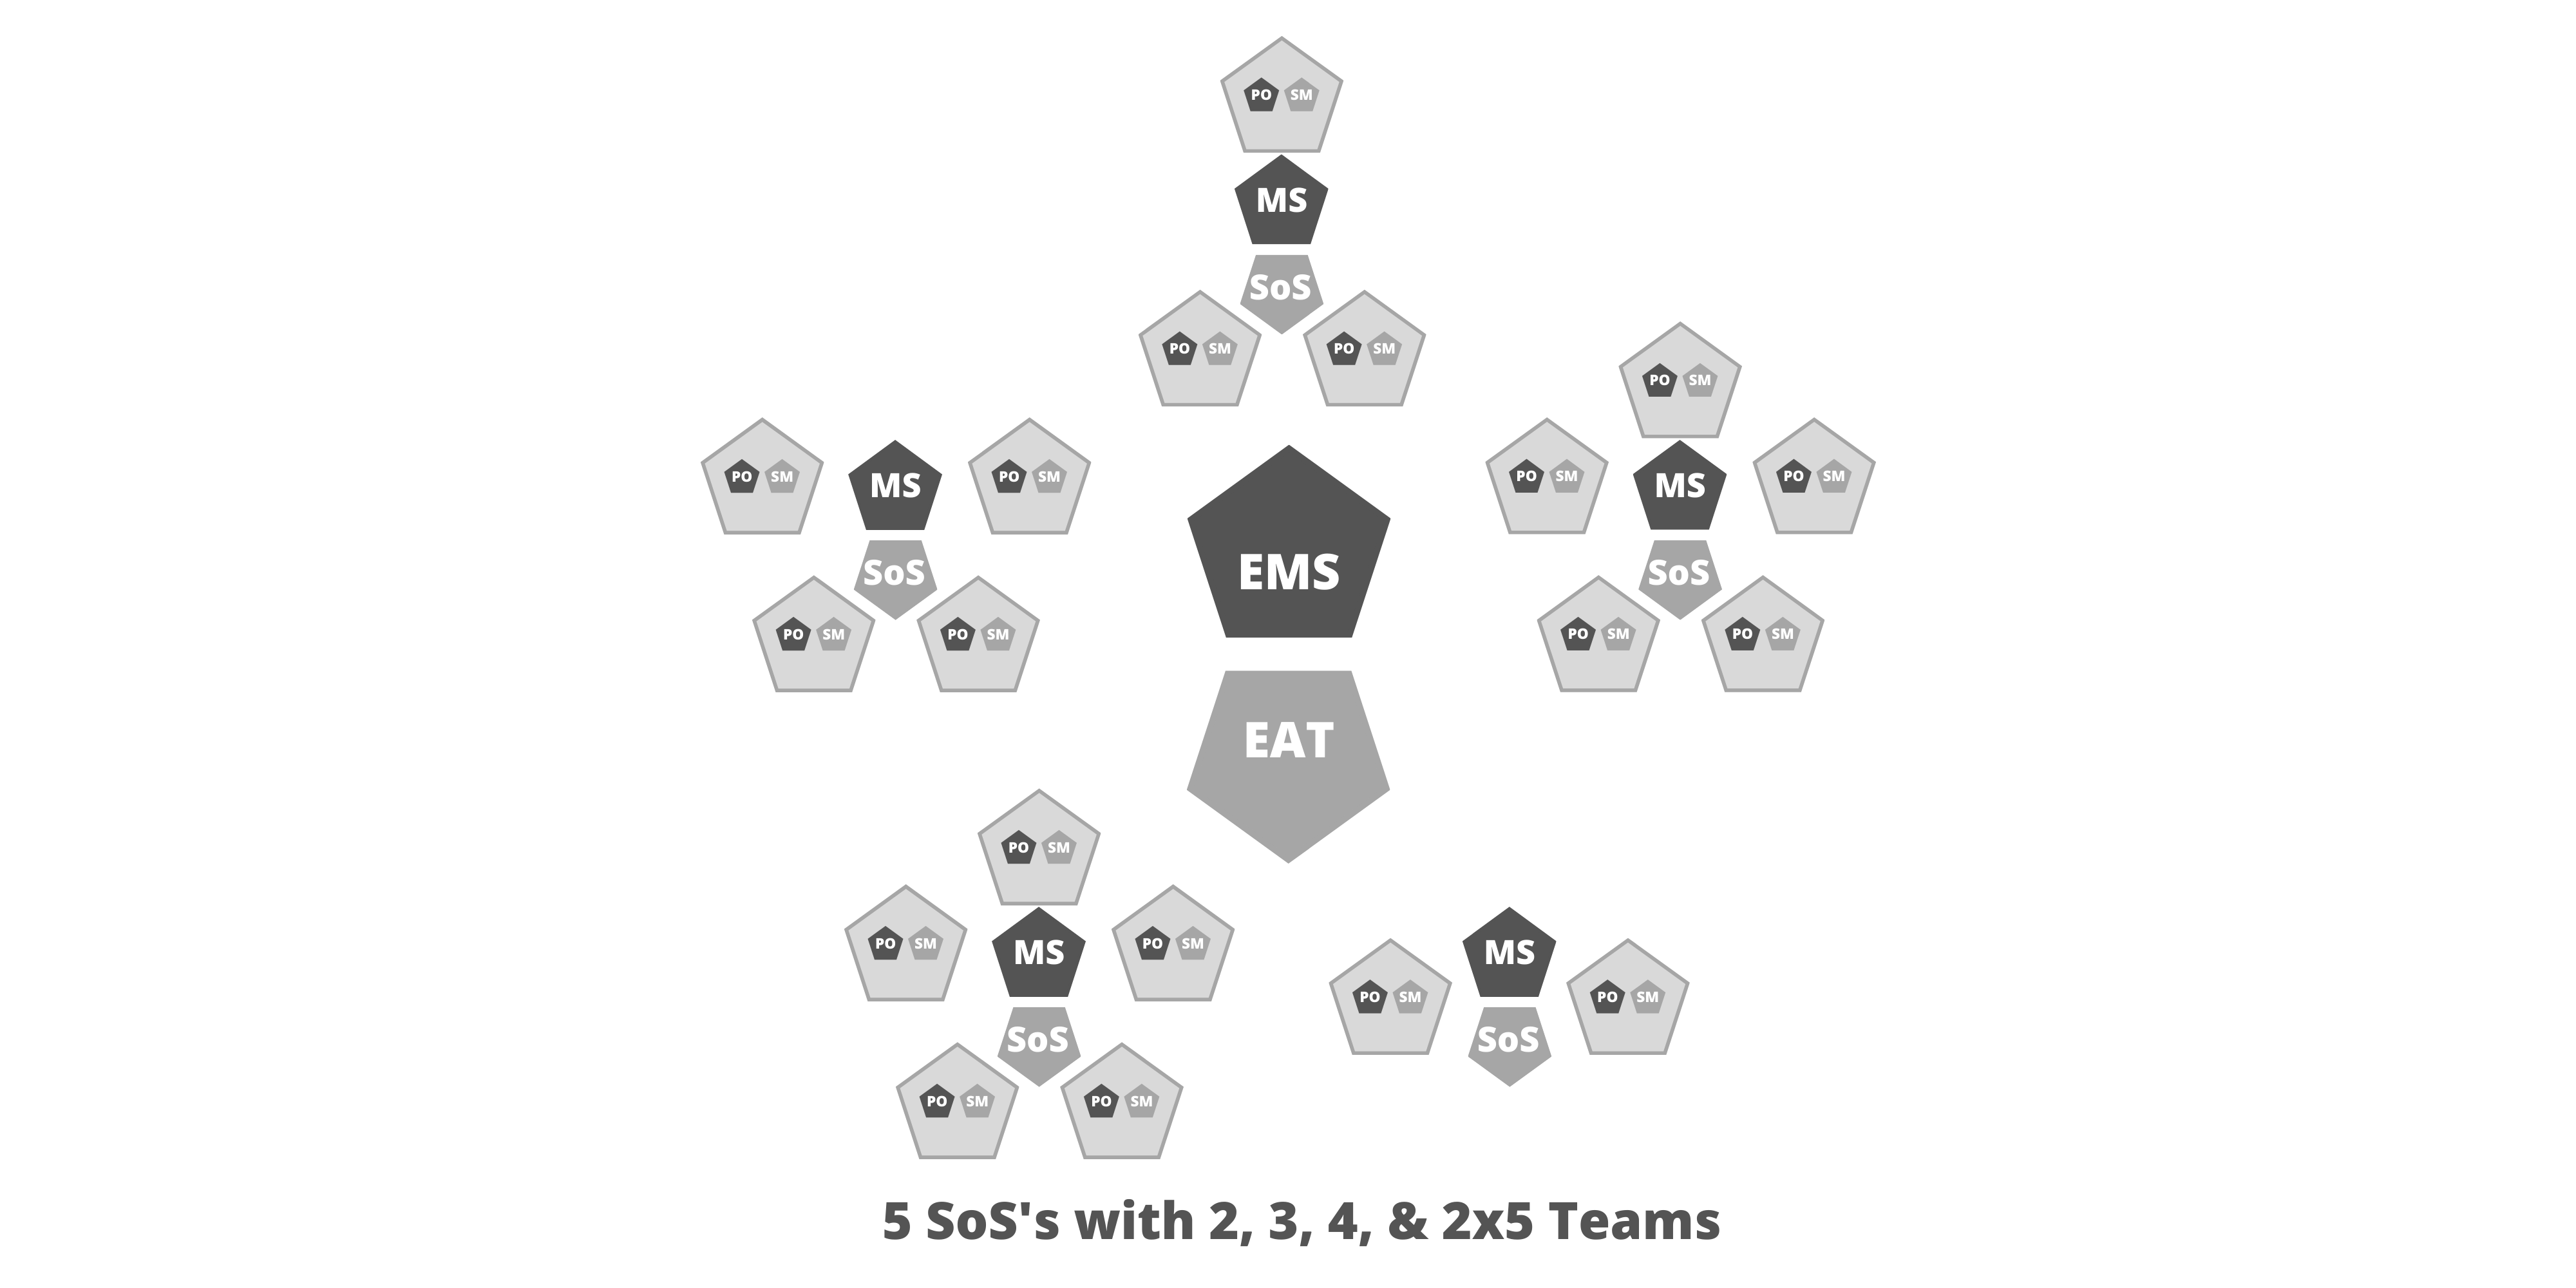
\includegraphics[scale=0.15]{4.png}
\end{figure}


\begin{figure}[H]
    \centering
    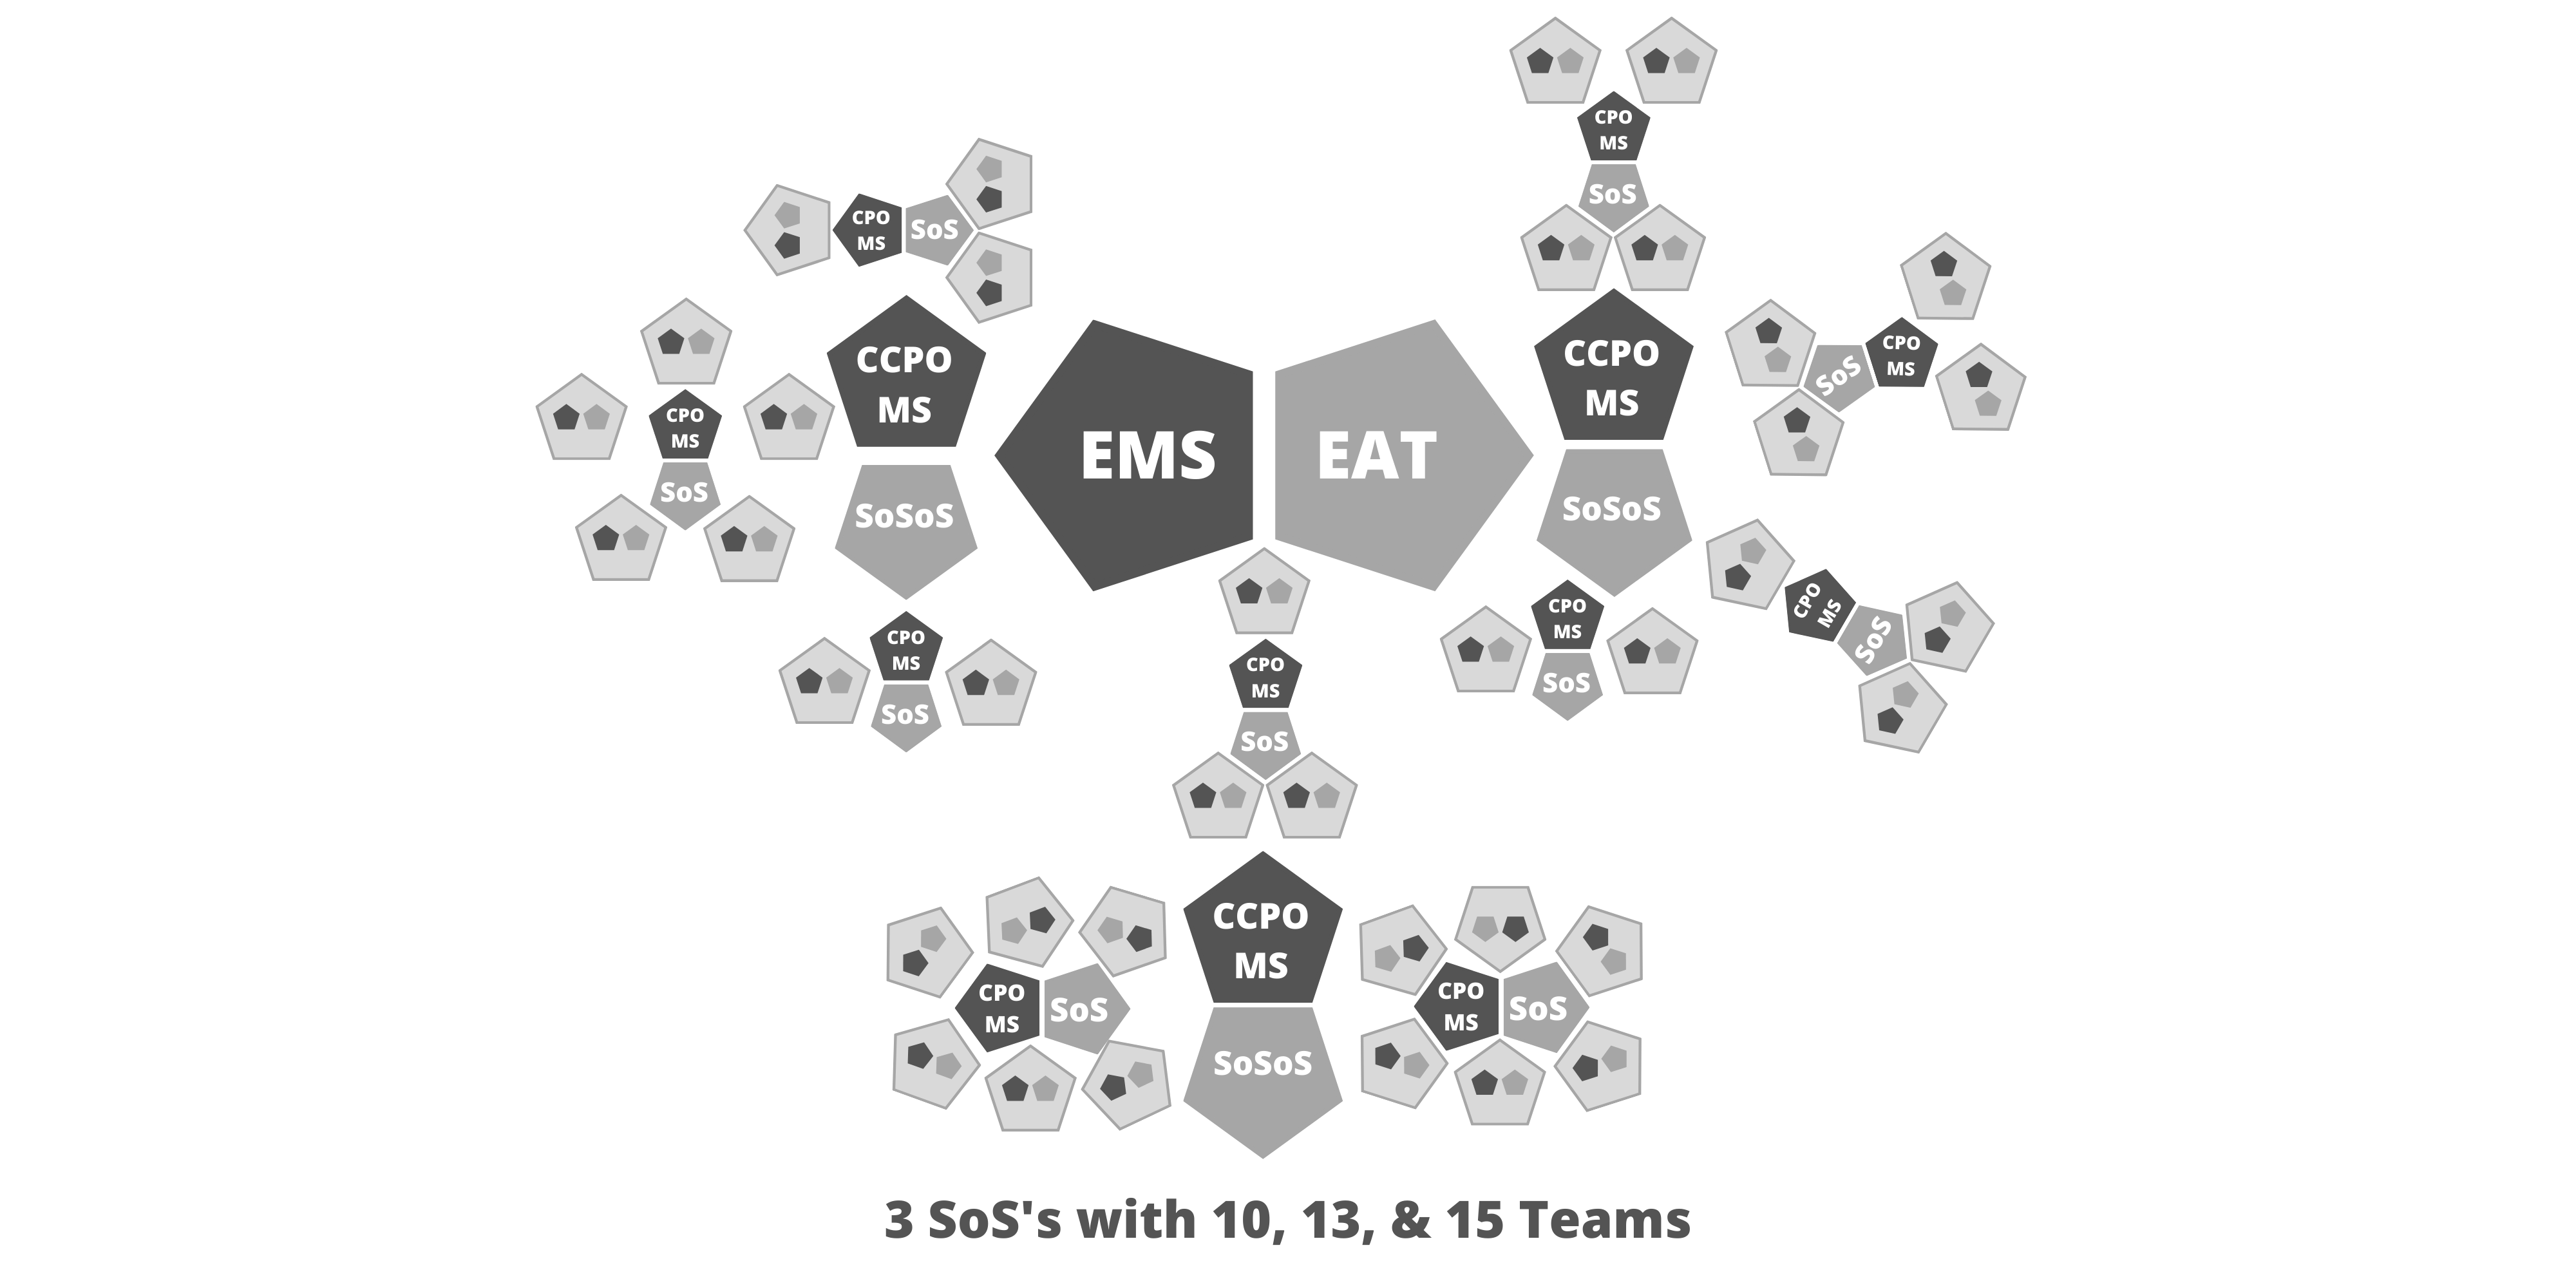
\includegraphics[scale=0.15]{5.png}
\end{figure}

\iffalse
Customer Relations, Legal / Compliance, and People Operations are included here since they are necessary parts of organizations and will exist as independent Scrum Teams on their own, upon which all other teams may rely.
\fi
カスタマーリレーションズ、法務/コンプライアンス、人事がこの図に含まれているのは、組織の必要な部分であり、他の全チームが頼る独立したスクラムチームとして存在するためである。

\iffalse
A final note on the representation of the Executive Action Team and the Executive MetaScrum: In this diagram, they are shown as overlapping since some members sit on both of the teams. In very small organizations or implementations, the Executive Action Team and the Executive MetaScrum may consist entirely of the same team members.
\fi
エグゼクティブアクションチームとエグゼクティブメタスクラムの表現に関する注記: この図では、一部のメンバーが両方のチームに在席しているため、重複して表現している。非常に小規模な組織や実装では、エグゼクティブアクションチームとエグゼクティブメタスクラムはまったく同じチームメンバーで構成されている場合がある。

\begin{figure}[H]
    \centering
    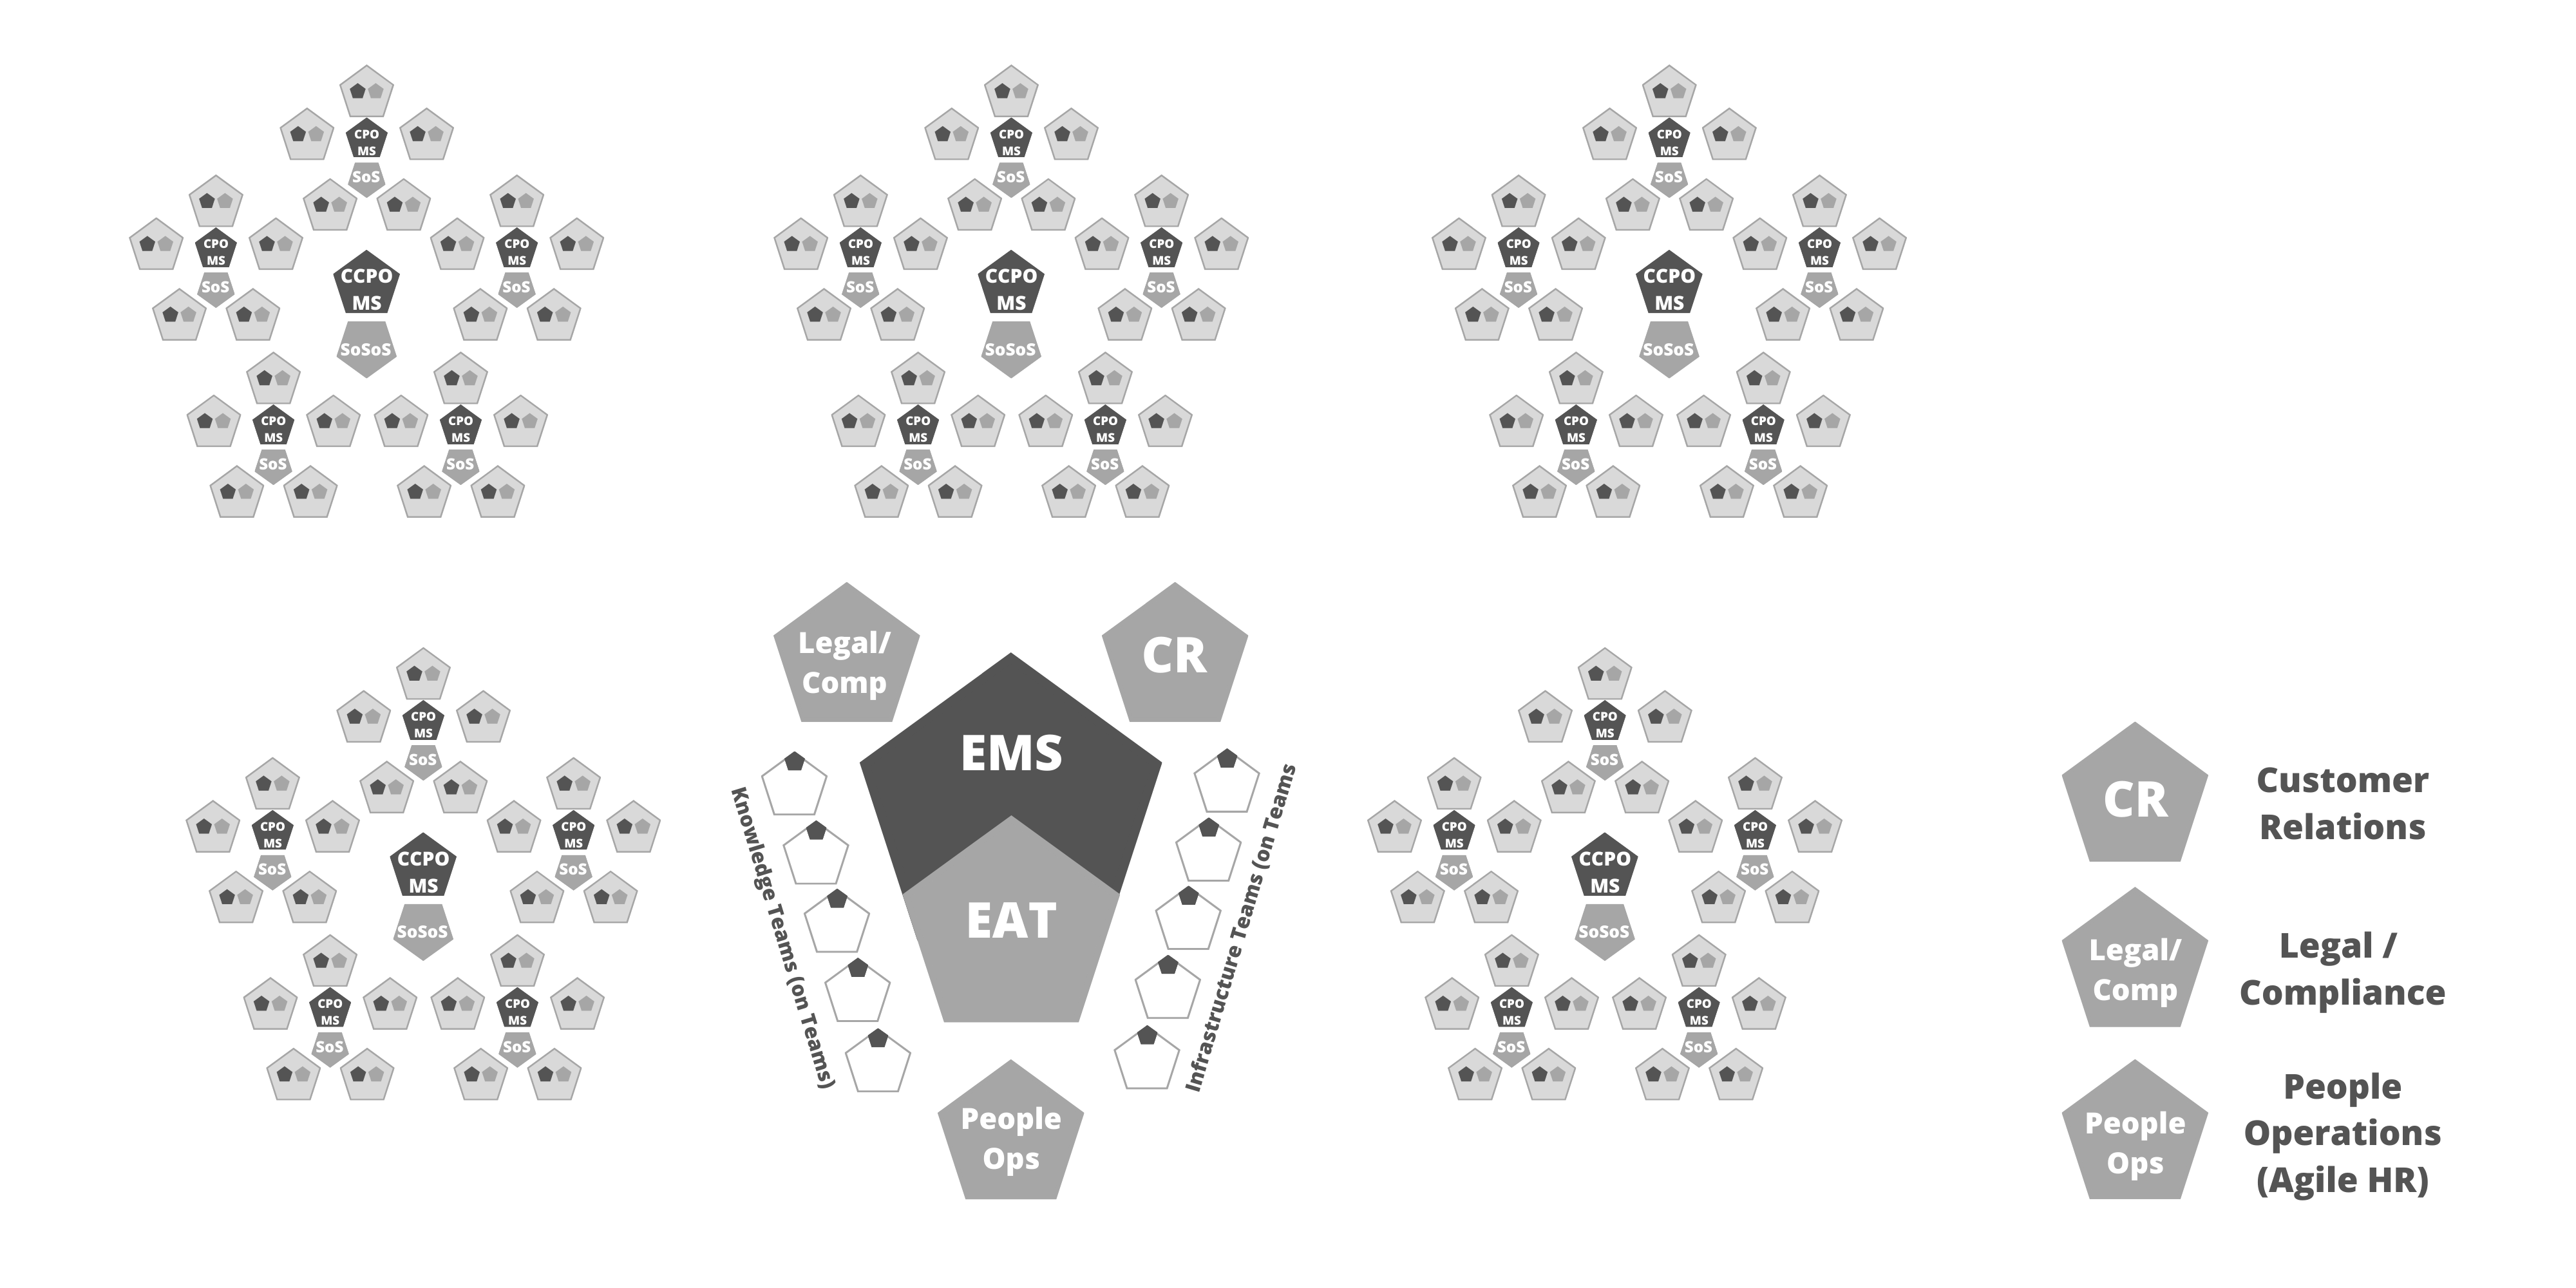
\includegraphics[scale=0.15]{6.png}
\end{figure}


\iffalse
\emph{In this organizational diagram, the Knowledge and Infrastructure Teams represent virtual teams of specialists of which there are too few to staff each team. If they act as shared-services team, they coordinate with the Scrum Teams as a group, where requests flow through a Product Owner for each specialty who converts them into a transparent prioritized backlog. An important note is that these teams are NOT silos of individuals who sit together (this is why they are represented as hollow pentagons); their team members sit on the actual Scrum Teams, but they make up this virtual Scrum of their own for the purpose of backlog dissemination and process improvement.}
\fi
この組織図では、ナレッジチームとインフラストラクチャチームは、各チームにスタッフを配置するには少なすぎる専門家の仮想チームを表している。仮想チームが、共通サービスを提供するチームとして機能する場合、グループとして周りのスクラムチームと調整する。周りのスクラムチームからの要求は各専門分野の仮想チームのプロダクトオーナーを経由して、透明性のある優先順位付けされたバックログとして管理される。重要な点は、仮想チームは、隣同士に座っている個人のサイロではないということである(白抜き五角形で表現されている理由)。仮想チームのチームメンバーは実際のスクラムチームに席を持っており、スプリント中はスクラムチームの一員となる。一方、バックログの配布とプロセスの改善のために、この仮想スクラムを独自に構成する。


\iffalse
\subsection{End Note}\label{End-Note}
\fi
\subsection{後書}\label{End-Note}

\iffalse
Scrum@Scale is designed to scale productivity, to get an entire
organization delivering twice the value at half the cost. Implementing a
streamlined workflow at a sustainable pace with better decision making
improves the work environment, increases business agility, and generates
higher returns to all stakeholders.
\fi
Scrum@Scaleは、生産性を向上させ、組織全体が半分のコストで2倍の価値を提供できるように設計されている。合理化されたワークフローを、持続可能なペースで実装し、優れた意思決定を行うと、作業環境が改善され、ビジネスのアジリティが高まり、すべてのステークホルダーにより高い利益がもたらされる。

\iffalse
Scrum@Scale is designed to saturate an organization with Scrum. Well
implemented Scrum can run an entire organization with Scrum@Scale as the
operating system.
\fi
Scrum@Scaleは、組織にスクラムを浸透させるように設計されている。スクラムをうまく実装すると、Scrum@Scaleをオペレーティングシステムとして使い、組織全体を運営することができる。

\iffalse
\subsection{Acknowledgements}\label{Acknowledgements}
\fi
\subsection{謝辞}\label{Acknowledgements}

\iffalse
\subsubsection{History}\label{History}
\fi
\subsubsection{歴史}\label{History}


\iffalse
Dr. Jeff Sutherland developed Scrum@Scale based on the fundamental principles behind Scrum, Complex Adaptive Systems theory, game theory, and his work in biology. The original version of this guide was created by collaboration with Jessica Larsen, Avi Schneier, and Alex Sutherland. Subsequent editions have been refined with the input of many experienced Scrum practitioners based on the results of their field work.
\fi
ジェフ・サザーランド博士は、スクラムの背後にある原則、複雑系適応システム理論、ゲーム理論、および生物学における彼の研究に基づきScrum@Scaleを開発した。本ガイドの原版は、Jessica Larsen、Avi Schneier、Alex Sutherlandの協力により作成された。以降の版は、多くの経験豊かなスクラムの実践者のフィールドワークの結果に基づいて改良されている。

\iffalse
\subsubsection{People and Organizations}\label{People-and-Organizations}
\fi
\subsubsection{人と組織}\label{People-and-Organizations}


\iffalse
We acknowledge IDX for the creation of the Scrum of Scrums which first
allowed Scrum to scale to hundreds of
teams\textsuperscript{\hyperref[citation6]{6}}, PatientKeeper for the
creation of the MetaScrum\textsuperscript{\hyperref[citation7]{7}},
which enabled rapid deployment of innovative product, and OpenView
Venture Partners for scaling Scrum to the entire
organization\textsuperscript{\hyperref[citation8]{8}}. We value input
from Intel, who taught us ``nothing scales except a scale-free
architecture'', and SAP, with the largest Scrum team product
organization, who taught us management involvement in the MetaScrum is
essential to get more than 2,000 Scrum Teams to work together.
\fi
我々は、IDX社において、スクラムを何百ものチームに広げることを最初に許してくれたことで、スクラムオブスクラムが生まれたと認識している\textsuperscript{\hyperref[citation6]{6}}。PentientKeeper社ではメタスクラムが生まれ\textsuperscript{\hyperref[citation7]{7}}、革新的な製品の高速開発を可能にし、OpenView Venture Partners社はスクラムを組織全体に拡大した\textsuperscript{\hyperref[citation8]{8}}。Intel社は、スケールフリーアーキテクチャ無しには "何もスケールしない”ことを私たちに教え、最大のスクラムチーム製品部門を持つSAP社は、2,000を超えるスクラムチームがともに働くためには、メタスクラムにおけるマネジメントの関与が必須であるということを教えてくれた。

\iffalse
The agile coaches and trainers implementing these concepts at Amazon, GE, 3M, Toyota, Spotify, Maersk, Comcast, AT\&T and many other companies have been helpful in testing these concepts across a wide range of businesses across different domains
\fi
Amazon、GE、3M、トヨタ、Spotify、Maersk、Comcast、AT\&Tなどの多くの企業でScrum@Scaleのコンセプトを導入しているアジャイルコーチとトレーナーたちは、異なるドメインの幅広い企業にまたがり、Scrum@Scaleのコンセプトをテストすることに協力し続けてくれている。

~
\pagebreak
\begin{center}\rule{3in}{0.4pt}\end{center}

\begin{enumerate}
\itemsep1pt\parskip0pt\parsep0pt
\iffalse
\item
  ``Business agility.'' Wikipedia, Last modified 27 February
  2020.
  \newline ~\href{https://en.wikipedia.org/wiki/Business_agility}{https://en.wikipedia.org/wiki/Business\_agility}.
\item
  Johnson, Jim. New CHAOS Report. The Standish Group. 2018.
\item
  Ogunnaike, Babatunde A. and Ray, W. Harmon. Process Dynamics, Modeling
  and Control. Oxford University Press. 1994.
\item
  Hackman, J Richard. Leading Teams: Setting the Stage for Great
  Performances. Harvard Business Press. 2002.
\item
  Sutherland, Jeff, Coplien, James O., and The Scrum Patterns Group. A
  Scrum Book: The Spirit of the Game. Pragmatic Bookshelf. 2019.
\item
  Sutherland, Jeff. ``Inventing and Reinventing SCRUM in five
  Companies.'' Sur le site officiel de l'alliance agile. 2001.
\item
  Sutherland, Jeff. ``Future of Scrum: Parallel Pipelining of Sprints in
  Complex Projects.'' Proceedings of the Agile Development Conference.
  IEEE Computer Society 90-102. 2005.
\item
  Sutherland, Jeff and Altman, Igor. ``Take No Prisoners: How a Venture
  Capital Group Does Scrum.'' Agile Conference, 2009. AGILE'09, IEEE
  350-355. 2009.
\fi
\item
  “Business agility(ビジネスのアジリティ)”、Wikipedia、最終変更2020年2月27日。
  \newline ~\href{https://en.wikipedia.org/wiki/Business_agility}{https://en.wikipedia.org/wiki/Business\_agility}.
\item
  Johnson, Jim、新カオスレポート、The Standish Group、2018年。
\item
  Ogunnaike, Babatunde A.、Ray, W. Harmon、Process Dynamics, Modeling and Control(プロセスのダイナミクス、モデル、制御)、Oxford University Press、1994年。
\item
  Hackman, J Richard、Leading Teams: Setting the Stage for Great Performances(チームをリードする: パフォーマンスを高めるステージの設定)、Harvard Business Press、2002年。
\item
  Sutherland, Jeff、Coplien, James O.、The Scrum Patterns Group、A Scrum Book: The Spirit of the Game(スクラムブック: ゲームのスピリット)、Pragmatic Bookshelf、2019年。
\item
  Sutherland, Jeff、“Inventing and Reinventing SCRUM in five Companies(5社におけるスクラムの発明と再発明)”、Sur le site officiel de l’alliance agile、2001年。
\item
  Sutherland, Jeff、“Future of Scrum: Parallel Pipelining of Sprints in Complex Projects(スクラムの未来: 複雑なプロジェクトにおけるスプリントの並行パイプライン化)”、Proceedings of the Agile Development Conference(アジャイル開発会議の内容)、IEEE Computer Society 90-102、2005年。
\item
  Sutherland, Jeff、Altman, Igor、“Take No Prisoners: How a Venture Capital Group Does Scrum(やってみよう: ベンチャーキャピタルグループでスクラムを実践する方法)”、Agile Conference(アジャイル会議)、2009年。AGILE’09, IEEE 350-355、2009年。
\end{enumerate}

\end{document}
